% setwd("E:/CODE/DISSERTATION") % be sure to run with 'Sweave2' # for normal sweave
% setwd("C:/Users/triffe/git/DISSERTATION_REPO/DISSERTATION") # for pgfsweave
\documentclass[reqno,12pt,oneside,a4paper]{report} % right-side equation numbering, 12 point font, print one-sided 
\newcommand{\hlnumber}[1]{\textcolor[rgb]{0.0823529411764706,0.0784313725490196,0.709803921568627}{#1}}%
\newcommand{\hlfunctioncall}[1]{\textcolor[rgb]{1,0,0}{#1}}%
\newcommand{\hlstring}[1]{\textcolor[rgb]{0.6,0.6,1}{#1}}%
\newcommand{\hlkeyword}[1]{\textcolor[rgb]{0,0,0}{\textbf{#1}}}%
\newcommand{\hlargument}[1]{\textcolor[rgb]{0.694117647058824,0.247058823529412,0.0196078431372549}{#1}}%
\newcommand{\hlcomment}[1]{\textcolor[rgb]{0.8,0.8,0.8}{#1}}%
\newcommand{\hlroxygencomment}[1]{\textcolor[rgb]{0,0.592156862745098,1}{#1}}%
\newcommand{\hlformalargs}[1]{\textcolor[rgb]{0.0705882352941176,0.713725490196078,0.0705882352941176}{#1}}%
\newcommand{\hleqformalargs}[1]{\textcolor[rgb]{0.0705882352941176,0.713725490196078,0.0705882352941176}{#1}}%
\newcommand{\hlassignement}[1]{\textcolor[rgb]{0.215686274509804,0.215686274509804,0.384313725490196}{\textbf{#1}}}%
\newcommand{\hlpackage}[1]{\textcolor[rgb]{0.588235294117647,0.713725490196078,0.145098039215686}{#1}}%
\newcommand{\hlslot}[1]{\textit{#1}}%
\newcommand{\hlsymbol}[1]{\textcolor[rgb]{0,0,0}{#1}}%
\newcommand{\hlprompt}[1]{\textcolor[rgb]{0,0,0}{#1}}%

\usepackage{color}%
 
\newsavebox{\hlnormalsizeboxclosebrace}%
\newsavebox{\hlnormalsizeboxopenbrace}%
\newsavebox{\hlnormalsizeboxbackslash}%
\newsavebox{\hlnormalsizeboxlessthan}%
\newsavebox{\hlnormalsizeboxgreaterthan}%
\newsavebox{\hlnormalsizeboxdollar}%
\newsavebox{\hlnormalsizeboxunderscore}%
\newsavebox{\hlnormalsizeboxand}%
\newsavebox{\hlnormalsizeboxhash}%
\newsavebox{\hlnormalsizeboxat}%
\newsavebox{\hlnormalsizeboxpercent}% 
\newsavebox{\hlnormalsizeboxhat}%
\newsavebox{\hlnormalsizeboxsinglequote}%
\newsavebox{\hlnormalsizeboxbacktick}%

\setbox\hlnormalsizeboxopenbrace=\hbox{\begin{normalsize}\verb.{.\end{normalsize}}%
\setbox\hlnormalsizeboxclosebrace=\hbox{\begin{normalsize}\verb.}.\end{normalsize}}%
\setbox\hlnormalsizeboxlessthan=\hbox{\begin{normalsize}\verb.<.\end{normalsize}}%
\setbox\hlnormalsizeboxdollar=\hbox{\begin{normalsize}\verb.$.\end{normalsize}}%
\setbox\hlnormalsizeboxunderscore=\hbox{\begin{normalsize}\verb._.\end{normalsize}}%
\setbox\hlnormalsizeboxand=\hbox{\begin{normalsize}\verb.&.\end{normalsize}}%
\setbox\hlnormalsizeboxhash=\hbox{\begin{normalsize}\verb.#.\end{normalsize}}%
\setbox\hlnormalsizeboxat=\hbox{\begin{normalsize}\verb.@.\end{normalsize}}%
\setbox\hlnormalsizeboxbackslash=\hbox{\begin{normalsize}\verb.\.\end{normalsize}}%
\setbox\hlnormalsizeboxgreaterthan=\hbox{\begin{normalsize}\verb.>.\end{normalsize}}%
\setbox\hlnormalsizeboxpercent=\hbox{\begin{normalsize}\verb.%.\end{normalsize}}%
\setbox\hlnormalsizeboxhat=\hbox{\begin{normalsize}\verb.^.\end{normalsize}}%
\setbox\hlnormalsizeboxsinglequote=\hbox{\begin{normalsize}\verb.'.\end{normalsize}}%
\setbox\hlnormalsizeboxbacktick=\hbox{\begin{normalsize}\verb.`.\end{normalsize}}%
\setbox\hlnormalsizeboxhat=\hbox{\begin{normalsize}\verb.^.\end{normalsize}}%



\newsavebox{\hltinyboxclosebrace}%
\newsavebox{\hltinyboxopenbrace}%
\newsavebox{\hltinyboxbackslash}%
\newsavebox{\hltinyboxlessthan}%
\newsavebox{\hltinyboxgreaterthan}%
\newsavebox{\hltinyboxdollar}%
\newsavebox{\hltinyboxunderscore}%
\newsavebox{\hltinyboxand}%
\newsavebox{\hltinyboxhash}%
\newsavebox{\hltinyboxat}%
\newsavebox{\hltinyboxpercent}% 
\newsavebox{\hltinyboxhat}%
\newsavebox{\hltinyboxsinglequote}%
\newsavebox{\hltinyboxbacktick}%

\setbox\hltinyboxopenbrace=\hbox{\begin{tiny}\verb.{.\end{tiny}}%
\setbox\hltinyboxclosebrace=\hbox{\begin{tiny}\verb.}.\end{tiny}}%
\setbox\hltinyboxlessthan=\hbox{\begin{tiny}\verb.<.\end{tiny}}%
\setbox\hltinyboxdollar=\hbox{\begin{tiny}\verb.$.\end{tiny}}%
\setbox\hltinyboxunderscore=\hbox{\begin{tiny}\verb._.\end{tiny}}%
\setbox\hltinyboxand=\hbox{\begin{tiny}\verb.&.\end{tiny}}%
\setbox\hltinyboxhash=\hbox{\begin{tiny}\verb.#.\end{tiny}}%
\setbox\hltinyboxat=\hbox{\begin{tiny}\verb.@.\end{tiny}}%
\setbox\hltinyboxbackslash=\hbox{\begin{tiny}\verb.\.\end{tiny}}%
\setbox\hltinyboxgreaterthan=\hbox{\begin{tiny}\verb.>.\end{tiny}}%
\setbox\hltinyboxpercent=\hbox{\begin{tiny}\verb.%.\end{tiny}}%
\setbox\hltinyboxhat=\hbox{\begin{tiny}\verb.^.\end{tiny}}%
\setbox\hltinyboxsinglequote=\hbox{\begin{tiny}\verb.'.\end{tiny}}%
\setbox\hltinyboxbacktick=\hbox{\begin{tiny}\verb.`.\end{tiny}}%
\setbox\hltinyboxhat=\hbox{\begin{tiny}\verb.^.\end{tiny}}%



\newsavebox{\hlscriptsizeboxclosebrace}%
\newsavebox{\hlscriptsizeboxopenbrace}%
\newsavebox{\hlscriptsizeboxbackslash}%
\newsavebox{\hlscriptsizeboxlessthan}%
\newsavebox{\hlscriptsizeboxgreaterthan}%
\newsavebox{\hlscriptsizeboxdollar}%
\newsavebox{\hlscriptsizeboxunderscore}%
\newsavebox{\hlscriptsizeboxand}%
\newsavebox{\hlscriptsizeboxhash}%
\newsavebox{\hlscriptsizeboxat}%
\newsavebox{\hlscriptsizeboxpercent}% 
\newsavebox{\hlscriptsizeboxhat}%
\newsavebox{\hlscriptsizeboxsinglequote}%
\newsavebox{\hlscriptsizeboxbacktick}%

\setbox\hlscriptsizeboxopenbrace=\hbox{\begin{scriptsize}\verb.{.\end{scriptsize}}%
\setbox\hlscriptsizeboxclosebrace=\hbox{\begin{scriptsize}\verb.}.\end{scriptsize}}%
\setbox\hlscriptsizeboxlessthan=\hbox{\begin{scriptsize}\verb.<.\end{scriptsize}}%
\setbox\hlscriptsizeboxdollar=\hbox{\begin{scriptsize}\verb.$.\end{scriptsize}}%
\setbox\hlscriptsizeboxunderscore=\hbox{\begin{scriptsize}\verb._.\end{scriptsize}}%
\setbox\hlscriptsizeboxand=\hbox{\begin{scriptsize}\verb.&.\end{scriptsize}}%
\setbox\hlscriptsizeboxhash=\hbox{\begin{scriptsize}\verb.#.\end{scriptsize}}%
\setbox\hlscriptsizeboxat=\hbox{\begin{scriptsize}\verb.@.\end{scriptsize}}%
\setbox\hlscriptsizeboxbackslash=\hbox{\begin{scriptsize}\verb.\.\end{scriptsize}}%
\setbox\hlscriptsizeboxgreaterthan=\hbox{\begin{scriptsize}\verb.>.\end{scriptsize}}%
\setbox\hlscriptsizeboxpercent=\hbox{\begin{scriptsize}\verb.%.\end{scriptsize}}%
\setbox\hlscriptsizeboxhat=\hbox{\begin{scriptsize}\verb.^.\end{scriptsize}}%
\setbox\hlscriptsizeboxsinglequote=\hbox{\begin{scriptsize}\verb.'.\end{scriptsize}}%
\setbox\hlscriptsizeboxbacktick=\hbox{\begin{scriptsize}\verb.`.\end{scriptsize}}%
\setbox\hlscriptsizeboxhat=\hbox{\begin{scriptsize}\verb.^.\end{scriptsize}}%



\newsavebox{\hlfootnotesizeboxclosebrace}%
\newsavebox{\hlfootnotesizeboxopenbrace}%
\newsavebox{\hlfootnotesizeboxbackslash}%
\newsavebox{\hlfootnotesizeboxlessthan}%
\newsavebox{\hlfootnotesizeboxgreaterthan}%
\newsavebox{\hlfootnotesizeboxdollar}%
\newsavebox{\hlfootnotesizeboxunderscore}%
\newsavebox{\hlfootnotesizeboxand}%
\newsavebox{\hlfootnotesizeboxhash}%
\newsavebox{\hlfootnotesizeboxat}%
\newsavebox{\hlfootnotesizeboxpercent}% 
\newsavebox{\hlfootnotesizeboxhat}%
\newsavebox{\hlfootnotesizeboxsinglequote}%
\newsavebox{\hlfootnotesizeboxbacktick}%

\setbox\hlfootnotesizeboxopenbrace=\hbox{\begin{footnotesize}\verb.{.\end{footnotesize}}%
\setbox\hlfootnotesizeboxclosebrace=\hbox{\begin{footnotesize}\verb.}.\end{footnotesize}}%
\setbox\hlfootnotesizeboxlessthan=\hbox{\begin{footnotesize}\verb.<.\end{footnotesize}}%
\setbox\hlfootnotesizeboxdollar=\hbox{\begin{footnotesize}\verb.$.\end{footnotesize}}%
\setbox\hlfootnotesizeboxunderscore=\hbox{\begin{footnotesize}\verb._.\end{footnotesize}}%
\setbox\hlfootnotesizeboxand=\hbox{\begin{footnotesize}\verb.&.\end{footnotesize}}%
\setbox\hlfootnotesizeboxhash=\hbox{\begin{footnotesize}\verb.#.\end{footnotesize}}%
\setbox\hlfootnotesizeboxat=\hbox{\begin{footnotesize}\verb.@.\end{footnotesize}}%
\setbox\hlfootnotesizeboxbackslash=\hbox{\begin{footnotesize}\verb.\.\end{footnotesize}}%
\setbox\hlfootnotesizeboxgreaterthan=\hbox{\begin{footnotesize}\verb.>.\end{footnotesize}}%
\setbox\hlfootnotesizeboxpercent=\hbox{\begin{footnotesize}\verb.%.\end{footnotesize}}%
\setbox\hlfootnotesizeboxhat=\hbox{\begin{footnotesize}\verb.^.\end{footnotesize}}%
\setbox\hlfootnotesizeboxsinglequote=\hbox{\begin{footnotesize}\verb.'.\end{footnotesize}}%
\setbox\hlfootnotesizeboxbacktick=\hbox{\begin{footnotesize}\verb.`.\end{footnotesize}}%
\setbox\hlfootnotesizeboxhat=\hbox{\begin{footnotesize}\verb.^.\end{footnotesize}}%



\newsavebox{\hlsmallboxclosebrace}%
\newsavebox{\hlsmallboxopenbrace}%
\newsavebox{\hlsmallboxbackslash}%
\newsavebox{\hlsmallboxlessthan}%
\newsavebox{\hlsmallboxgreaterthan}%
\newsavebox{\hlsmallboxdollar}%
\newsavebox{\hlsmallboxunderscore}%
\newsavebox{\hlsmallboxand}%
\newsavebox{\hlsmallboxhash}%
\newsavebox{\hlsmallboxat}%
\newsavebox{\hlsmallboxpercent}% 
\newsavebox{\hlsmallboxhat}%
\newsavebox{\hlsmallboxsinglequote}%
\newsavebox{\hlsmallboxbacktick}%

\setbox\hlsmallboxopenbrace=\hbox{\begin{small}\verb.{.\end{small}}%
\setbox\hlsmallboxclosebrace=\hbox{\begin{small}\verb.}.\end{small}}%
\setbox\hlsmallboxlessthan=\hbox{\begin{small}\verb.<.\end{small}}%
\setbox\hlsmallboxdollar=\hbox{\begin{small}\verb.$.\end{small}}%
\setbox\hlsmallboxunderscore=\hbox{\begin{small}\verb._.\end{small}}%
\setbox\hlsmallboxand=\hbox{\begin{small}\verb.&.\end{small}}%
\setbox\hlsmallboxhash=\hbox{\begin{small}\verb.#.\end{small}}%
\setbox\hlsmallboxat=\hbox{\begin{small}\verb.@.\end{small}}%
\setbox\hlsmallboxbackslash=\hbox{\begin{small}\verb.\.\end{small}}%
\setbox\hlsmallboxgreaterthan=\hbox{\begin{small}\verb.>.\end{small}}%
\setbox\hlsmallboxpercent=\hbox{\begin{small}\verb.%.\end{small}}%
\setbox\hlsmallboxhat=\hbox{\begin{small}\verb.^.\end{small}}%
\setbox\hlsmallboxsinglequote=\hbox{\begin{small}\verb.'.\end{small}}%
\setbox\hlsmallboxbacktick=\hbox{\begin{small}\verb.`.\end{small}}%
\setbox\hlsmallboxhat=\hbox{\begin{small}\verb.^.\end{small}}%



\newsavebox{\hllargeboxclosebrace}%
\newsavebox{\hllargeboxopenbrace}%
\newsavebox{\hllargeboxbackslash}%
\newsavebox{\hllargeboxlessthan}%
\newsavebox{\hllargeboxgreaterthan}%
\newsavebox{\hllargeboxdollar}%
\newsavebox{\hllargeboxunderscore}%
\newsavebox{\hllargeboxand}%
\newsavebox{\hllargeboxhash}%
\newsavebox{\hllargeboxat}%
\newsavebox{\hllargeboxpercent}% 
\newsavebox{\hllargeboxhat}%
\newsavebox{\hllargeboxsinglequote}%
\newsavebox{\hllargeboxbacktick}%

\setbox\hllargeboxopenbrace=\hbox{\begin{large}\verb.{.\end{large}}%
\setbox\hllargeboxclosebrace=\hbox{\begin{large}\verb.}.\end{large}}%
\setbox\hllargeboxlessthan=\hbox{\begin{large}\verb.<.\end{large}}%
\setbox\hllargeboxdollar=\hbox{\begin{large}\verb.$.\end{large}}%
\setbox\hllargeboxunderscore=\hbox{\begin{large}\verb._.\end{large}}%
\setbox\hllargeboxand=\hbox{\begin{large}\verb.&.\end{large}}%
\setbox\hllargeboxhash=\hbox{\begin{large}\verb.#.\end{large}}%
\setbox\hllargeboxat=\hbox{\begin{large}\verb.@.\end{large}}%
\setbox\hllargeboxbackslash=\hbox{\begin{large}\verb.\.\end{large}}%
\setbox\hllargeboxgreaterthan=\hbox{\begin{large}\verb.>.\end{large}}%
\setbox\hllargeboxpercent=\hbox{\begin{large}\verb.%.\end{large}}%
\setbox\hllargeboxhat=\hbox{\begin{large}\verb.^.\end{large}}%
\setbox\hllargeboxsinglequote=\hbox{\begin{large}\verb.'.\end{large}}%
\setbox\hllargeboxbacktick=\hbox{\begin{large}\verb.`.\end{large}}%
\setbox\hllargeboxhat=\hbox{\begin{large}\verb.^.\end{large}}%



\newsavebox{\hlLargeboxclosebrace}%
\newsavebox{\hlLargeboxopenbrace}%
\newsavebox{\hlLargeboxbackslash}%
\newsavebox{\hlLargeboxlessthan}%
\newsavebox{\hlLargeboxgreaterthan}%
\newsavebox{\hlLargeboxdollar}%
\newsavebox{\hlLargeboxunderscore}%
\newsavebox{\hlLargeboxand}%
\newsavebox{\hlLargeboxhash}%
\newsavebox{\hlLargeboxat}%
\newsavebox{\hlLargeboxpercent}% 
\newsavebox{\hlLargeboxhat}%
\newsavebox{\hlLargeboxsinglequote}%
\newsavebox{\hlLargeboxbacktick}%

\setbox\hlLargeboxopenbrace=\hbox{\begin{Large}\verb.{.\end{Large}}%
\setbox\hlLargeboxclosebrace=\hbox{\begin{Large}\verb.}.\end{Large}}%
\setbox\hlLargeboxlessthan=\hbox{\begin{Large}\verb.<.\end{Large}}%
\setbox\hlLargeboxdollar=\hbox{\begin{Large}\verb.$.\end{Large}}%
\setbox\hlLargeboxunderscore=\hbox{\begin{Large}\verb._.\end{Large}}%
\setbox\hlLargeboxand=\hbox{\begin{Large}\verb.&.\end{Large}}%
\setbox\hlLargeboxhash=\hbox{\begin{Large}\verb.#.\end{Large}}%
\setbox\hlLargeboxat=\hbox{\begin{Large}\verb.@.\end{Large}}%
\setbox\hlLargeboxbackslash=\hbox{\begin{Large}\verb.\.\end{Large}}%
\setbox\hlLargeboxgreaterthan=\hbox{\begin{Large}\verb.>.\end{Large}}%
\setbox\hlLargeboxpercent=\hbox{\begin{Large}\verb.%.\end{Large}}%
\setbox\hlLargeboxhat=\hbox{\begin{Large}\verb.^.\end{Large}}%
\setbox\hlLargeboxsinglequote=\hbox{\begin{Large}\verb.'.\end{Large}}%
\setbox\hlLargeboxbacktick=\hbox{\begin{Large}\verb.`.\end{Large}}%
\setbox\hlLargeboxhat=\hbox{\begin{Large}\verb.^.\end{Large}}%



\newsavebox{\hlLARGEboxclosebrace}%
\newsavebox{\hlLARGEboxopenbrace}%
\newsavebox{\hlLARGEboxbackslash}%
\newsavebox{\hlLARGEboxlessthan}%
\newsavebox{\hlLARGEboxgreaterthan}%
\newsavebox{\hlLARGEboxdollar}%
\newsavebox{\hlLARGEboxunderscore}%
\newsavebox{\hlLARGEboxand}%
\newsavebox{\hlLARGEboxhash}%
\newsavebox{\hlLARGEboxat}%
\newsavebox{\hlLARGEboxpercent}% 
\newsavebox{\hlLARGEboxhat}%
\newsavebox{\hlLARGEboxsinglequote}%
\newsavebox{\hlLARGEboxbacktick}%

\setbox\hlLARGEboxopenbrace=\hbox{\begin{LARGE}\verb.{.\end{LARGE}}%
\setbox\hlLARGEboxclosebrace=\hbox{\begin{LARGE}\verb.}.\end{LARGE}}%
\setbox\hlLARGEboxlessthan=\hbox{\begin{LARGE}\verb.<.\end{LARGE}}%
\setbox\hlLARGEboxdollar=\hbox{\begin{LARGE}\verb.$.\end{LARGE}}%
\setbox\hlLARGEboxunderscore=\hbox{\begin{LARGE}\verb._.\end{LARGE}}%
\setbox\hlLARGEboxand=\hbox{\begin{LARGE}\verb.&.\end{LARGE}}%
\setbox\hlLARGEboxhash=\hbox{\begin{LARGE}\verb.#.\end{LARGE}}%
\setbox\hlLARGEboxat=\hbox{\begin{LARGE}\verb.@.\end{LARGE}}%
\setbox\hlLARGEboxbackslash=\hbox{\begin{LARGE}\verb.\.\end{LARGE}}%
\setbox\hlLARGEboxgreaterthan=\hbox{\begin{LARGE}\verb.>.\end{LARGE}}%
\setbox\hlLARGEboxpercent=\hbox{\begin{LARGE}\verb.%.\end{LARGE}}%
\setbox\hlLARGEboxhat=\hbox{\begin{LARGE}\verb.^.\end{LARGE}}%
\setbox\hlLARGEboxsinglequote=\hbox{\begin{LARGE}\verb.'.\end{LARGE}}%
\setbox\hlLARGEboxbacktick=\hbox{\begin{LARGE}\verb.`.\end{LARGE}}%
\setbox\hlLARGEboxhat=\hbox{\begin{LARGE}\verb.^.\end{LARGE}}%



\newsavebox{\hlhugeboxclosebrace}%
\newsavebox{\hlhugeboxopenbrace}%
\newsavebox{\hlhugeboxbackslash}%
\newsavebox{\hlhugeboxlessthan}%
\newsavebox{\hlhugeboxgreaterthan}%
\newsavebox{\hlhugeboxdollar}%
\newsavebox{\hlhugeboxunderscore}%
\newsavebox{\hlhugeboxand}%
\newsavebox{\hlhugeboxhash}%
\newsavebox{\hlhugeboxat}%
\newsavebox{\hlhugeboxpercent}% 
\newsavebox{\hlhugeboxhat}%
\newsavebox{\hlhugeboxsinglequote}%
\newsavebox{\hlhugeboxbacktick}%

\setbox\hlhugeboxopenbrace=\hbox{\begin{huge}\verb.{.\end{huge}}%
\setbox\hlhugeboxclosebrace=\hbox{\begin{huge}\verb.}.\end{huge}}%
\setbox\hlhugeboxlessthan=\hbox{\begin{huge}\verb.<.\end{huge}}%
\setbox\hlhugeboxdollar=\hbox{\begin{huge}\verb.$.\end{huge}}%
\setbox\hlhugeboxunderscore=\hbox{\begin{huge}\verb._.\end{huge}}%
\setbox\hlhugeboxand=\hbox{\begin{huge}\verb.&.\end{huge}}%
\setbox\hlhugeboxhash=\hbox{\begin{huge}\verb.#.\end{huge}}%
\setbox\hlhugeboxat=\hbox{\begin{huge}\verb.@.\end{huge}}%
\setbox\hlhugeboxbackslash=\hbox{\begin{huge}\verb.\.\end{huge}}%
\setbox\hlhugeboxgreaterthan=\hbox{\begin{huge}\verb.>.\end{huge}}%
\setbox\hlhugeboxpercent=\hbox{\begin{huge}\verb.%.\end{huge}}%
\setbox\hlhugeboxhat=\hbox{\begin{huge}\verb.^.\end{huge}}%
\setbox\hlhugeboxsinglequote=\hbox{\begin{huge}\verb.'.\end{huge}}%
\setbox\hlhugeboxbacktick=\hbox{\begin{huge}\verb.`.\end{huge}}%
\setbox\hlhugeboxhat=\hbox{\begin{huge}\verb.^.\end{huge}}%



\newsavebox{\hlHugeboxclosebrace}%
\newsavebox{\hlHugeboxopenbrace}%
\newsavebox{\hlHugeboxbackslash}%
\newsavebox{\hlHugeboxlessthan}%
\newsavebox{\hlHugeboxgreaterthan}%
\newsavebox{\hlHugeboxdollar}%
\newsavebox{\hlHugeboxunderscore}%
\newsavebox{\hlHugeboxand}%
\newsavebox{\hlHugeboxhash}%
\newsavebox{\hlHugeboxat}%
\newsavebox{\hlHugeboxpercent}% 
\newsavebox{\hlHugeboxhat}%
\newsavebox{\hlHugeboxsinglequote}%
\newsavebox{\hlHugeboxbacktick}%

\setbox\hlHugeboxopenbrace=\hbox{\begin{Huge}\verb.{.\end{Huge}}%
\setbox\hlHugeboxclosebrace=\hbox{\begin{Huge}\verb.}.\end{Huge}}%
\setbox\hlHugeboxlessthan=\hbox{\begin{Huge}\verb.<.\end{Huge}}%
\setbox\hlHugeboxdollar=\hbox{\begin{Huge}\verb.$.\end{Huge}}%
\setbox\hlHugeboxunderscore=\hbox{\begin{Huge}\verb._.\end{Huge}}%
\setbox\hlHugeboxand=\hbox{\begin{Huge}\verb.&.\end{Huge}}%
\setbox\hlHugeboxhash=\hbox{\begin{Huge}\verb.#.\end{Huge}}%
\setbox\hlHugeboxat=\hbox{\begin{Huge}\verb.@.\end{Huge}}%
\setbox\hlHugeboxbackslash=\hbox{\begin{Huge}\verb.\.\end{Huge}}%
\setbox\hlHugeboxgreaterthan=\hbox{\begin{Huge}\verb.>.\end{Huge}}%
\setbox\hlHugeboxpercent=\hbox{\begin{Huge}\verb.%.\end{Huge}}%
\setbox\hlHugeboxhat=\hbox{\begin{Huge}\verb.^.\end{Huge}}%
\setbox\hlHugeboxsinglequote=\hbox{\begin{Huge}\verb.'.\end{Huge}}%
\setbox\hlHugeboxbacktick=\hbox{\begin{Huge}\verb.`.\end{Huge}}%
\setbox\hlHugeboxhat=\hbox{\begin{Huge}\verb.^.\end{Huge}}%
 

\def\urltilda{\kern -.15em\lower .7ex\hbox{\~{}}\kern .04em}%

\newcommand{\hlstd}[1]{\textcolor[rgb]{0,0,0}{#1}}%
\newcommand{\hlnum}[1]{\textcolor[rgb]{0.16,0.16,1}{#1}}
\newcommand{\hlesc}[1]{\textcolor[rgb]{1,0,1}{#1}}
\newcommand{\hlstr}[1]{\textcolor[rgb]{1,0,0}{#1}}
\newcommand{\hldstr}[1]{\textcolor[rgb]{0.51,0.51,0}{#1}}
\newcommand{\hlslc}[1]{\textcolor[rgb]{0.51,0.51,0.51}{\it{#1}}}
\newcommand{\hlcom}[1]{\textcolor[rgb]{0.51,0.51,0.51}{\it{#1}}}
\newcommand{\hldir}[1]{\textcolor[rgb]{0,0.51,0}{#1}}
\newcommand{\hlsym}[1]{\textcolor[rgb]{0,0,0}{#1}}
\newcommand{\hlline}[1]{\textcolor[rgb]{0.33,0.33,0.33}{#1}}
\newcommand{\hlkwa}[1]{\textcolor[rgb]{0,0,0}{\bf{#1}}}
\newcommand{\hlkwb}[1]{\textcolor[rgb]{0.51,0,0}{#1}}
\newcommand{\hlkwc}[1]{\textcolor[rgb]{0,0,0}{\bf{#1}}}
\newcommand{\hlkwd}[1]{\textcolor[rgb]{0,0,0.51}{#1}}

\newenvironment{Houtput}{\raggedright}{%
%
}
%\documentclass[reqno,12pt,twoside,openright]{report} % right-side equation numbering, 12 point font, print two-sided, Chapters start on odd pages. Rackham only accepts one-sided, so this is for personal printings.

\usepackage{uab}         % Use UAB thesis style file
\usepackage{aas_macros}  % To allow the reading of ADS journal references in the bibliography
\usepackage[intlimits]{amsmath} % Puts the limits of integrals on top and bottom
\usepackage{amsxtra}     % Use various AMS packages
\usepackage{amsthm}
\usepackage{amssymb}
\usepackage{amsfonts}
\usepackage{graphicx}    % Add some packages for figures. Read epslatex.pdf on ctan.tug.org
\usepackage{rotating}
\usepackage{color}
\usepackage{epsfig}
\usepackage{subfigure}   % To make subfigures. Read subfigure.pdf on ctan.tug.org
\usepackage{verbatim}
\usepackage{natbib}      % Allows you to use BibTeX
% some custom citation aliases
\defcitealias{rackham1947trans}{\textit{Aristotle}, Nichomachean Ethics, Book II, Chapter 6, Sections 4-5.}

\usepackage[printonlyused]{acronym} % For the List of Abbreviations. Read acronym.pdf on ctan.tug.org
\usepackage{setspace}    % Allows you to specify the line spacing
\doublespacing           % \onehalfspacing for 1.5 spacing, \doublespacing for 2.0 spacing.
\newcommand{\sun}{\ensuremath{\odot}} % sun symbol is \sun
%\usepackage{leftidx}     % for better left subscripts
\usepackage{fixltx2e}     % in-text subscripting, no math
%\usepackage[OT1]{fontenc}
\usepackage{bm}
%%%%%%%%%%%%%%%%%%%%%%%%%%%%%%%%%%%%%%%%%%%%%%%%%%%%%%%%%%%%%%%%%%%%%%%%%%%%%%%

% Various theorem environments. All of the following have the same numbering
% system as theorem.

\theoremstyle{plain}
\newtheorem{theorem}{Theorem}
\newtheorem{prop}[theorem]{Proposition}
\newtheorem{corollary}[theorem]{Corollary}
\newtheorem{lemma}[theorem]{Lemma}
\newtheorem{question}[theorem]{Question}
\newtheorem{conjecture}[theorem]{Conjecture}
\newtheorem{assumption}[theorem]{Assumption}

\theoremstyle{definition}
\newtheorem{definition}[theorem]{Definition}
\newtheorem{notation}[theorem]{Notation}
\newtheorem{condition}[theorem]{Condition}
\newtheorem{example}[theorem]{Example}
\newtheorem{introduction}[theorem]{Introduction}

\theoremstyle{remark}
\newtheorem{remark}[theorem]{Remark}
%%%%%%%%%%%%%%%%%%%%%%%%%%%%%%%%%%%%%%%%%%%%%%%%%%%%%%%%%%%%%%%%%%%%%%%%%%%%%%%

\numberwithin{theorem}{chapter}     % Numbers theorems "x.y" where x
                                    % is the section number, y is the
                                    % theorem number

%\renewcommand{\thetheorem}{\arabic{chapter}.\arabic{theorem}}

%\makeatletter                      % This sequence of commands will
%\let\c@equation\c@theorem          % incorporate equation numbering
%\makeatother                       % into the theorem numbering scheme

%\renewcommand{\theenumi}{(\roman{enumi})}

%%%%%%%%%%%%%%%%%%%%%%%%%%%%%%%%%%%%%%%%%%%%%%%%%%%%%%%%%%%%%%%%%%%%%%%%%%%%%%
% tidy is grat, just need to figure out how to optionally display console results...
\usepackage{Sweave}

\usepackage{tikz}
\usetikzlibrary{external}
\tikzexternalize[mode=list and make]


% makes code more compact, changes indentation of code chunks
\DefineVerbatimEnvironment{Sinput}{Verbatim} {xleftmargin=2em}
\DefineVerbatimEnvironment{Soutput}{Verbatim}{xleftmargin=2em}
\DefineVerbatimEnvironment{Scode}{Verbatim}{xleftmargin=2em}
\fvset{listparameters={\setlength{\topsep}{0pt}}}
\renewenvironment{Schunk}{\vspace{\topsep}}{\vspace{\topsep}}

%%%%%%%%%%%%%%%%%%%%%%%%%%%%%%%%%%%%%%%%%%%%%%%%%%%%%%%%%%%%%%%%%%%%%%%%%%%%%%%
% If printing two-sided, this makes sure that any blank page at the 
% end of a chapter will not have a page number. 
\makeatletter
\def\cleardoublepage{\clearpage\if@twoside \ifodd\c@page\else
\hbox{}
\thispagestyle{empty}
\newpage
\if@twocolumn\hbox{}\newpage\fi\fi\fi}
\makeatother 

%%%%%%%%%%%%%%%%%%%%%%%%%%%%%%%%%%%%%%%%%%%%%%%%%%%%%%%%%%%%%%%%%%%%%%%%%%%%%%

%This command creates a box marked ``To Do'' around text.
%To use type \todo{  insert text here  }.

\newcommand{\todo}[1]{\vspace{5 mm}\par \noindent
\marginpar{\textsc{To Do}}
\framebox{\begin{minipage}[c]{0.95 \textwidth}
\tt\begin{center} #1 \end{center}\end{minipage}}\vspace{5 mm}\par}

%%%%%%%%%%%%%%%%%%%%%%%%%%%%%%%%%%%%%%%%%%%%%%%%%%%%%%%%%%%%%%%%%%%%%%%%%%%%%%%

%%%%%%%%%%%%%%%%%%%%%%%%%%%%%%%%%%%%%%%%%%%%%%%%%%%%%%%%%%%%%%%%%%%%%%%%%%%%%%%

%%%%%%%%%%%%%%%%%%%%%%%%%%%%%%%%%%%%%%%%%%%%%%%%%%%%%%%%%%%%%%%%%%%%%%%%%%%%%%%
\begin{document}

% this is to cache values produced in R to time recompiling code that contains calucations.


\bibliographystyle{agu04}    % Set the bibliography style. agu04, plain, alpha, etc.

% Title page 
\titlepage{The Two-Sex Problem in Demography}{Timothy L. M. Riffe}{Doctor of Philosophy}
{Program in Demography}{2013}
{Dr. Albert Esteve Pal\'{o}s, Chair\\
 Dr. Daniel Devolder\\
 Dr. Jane Demographer\\
 Dr. Joe Demographer\\
 Dr. Mike Demographer}

% Begin the front matter as required by Rackham dissertation guidelines
\initializefrontsections

% Optional Frontispiece
%\frontispiece{\includegraphics[width=6in]{Intro/Happy} Find a cool picture to go here.}

% Optional, but recommended, Copyright page
\copyrightpage{Timothy L. M. Riffe}

% Page numbering. If you don't include a frontispiece or copyright page, you'll need to change this for two-sided printing.
\makeatletter
\if@twoside \setcounter{page}{4} \else \setcounter{page}{1} \fi
\makeatother
 
% Optional Dedication page
\dedicationpage{For all the people}

% Optional Acknowledgements page
\startacknowledgementspage
% 
Many thanks to my teachers, classmates and colleagues for keeping me on my toes; the Ag\`{e}ncia de Gesti\'{o} d'Ajuts 
Universitaris i de Recerca of Catalunya, to the Centre d'Estudis Demogr\`{a}fics to the WorldFam project and the Ministerio de Educaci\'{o}n of Spain, 
for having financed all of my academic development from the fall of 2008 until the end of 2012. 
\label{Acknowledgements}

% Optional Preface page
%\startprefacepage
%\input{Preface}
%\label{Preface}

% Table of contents, list of figures, etc.
\tableofcontents     % Required
\listoffigures       % Required if there is more than one figure
%\listoftables        % Required if there is more than one table
%\listofmaps          % Required if there is more than one map
%\listofappendices    % Required if there is more than one appendix
%\listofabbreviations % Optional. Abbreviations should be stored in a file named abbr.tex

% Inserts abstract from external Rnw file
\startabstractpage
{The Two-Sex Problem in Demography}{Timothy L. M. Riffe}{Chair: Dr. Albert Esteve}
% shoot for 150 words
The most widely used measures and models of population formally assume fertility as a function of females only, 
'female dominance'. Early formal demographers proposed presently used indicators, such as $R_{0}$ and TFR as 
approximations, and accepted the assumption of female dominance as a matter of convenience rather than conviction.
 The magnitude and direction of error in measures of fertility and reproductivity due to this practice are not 
 always clear. Various adjustment procedures have been proposed in the past several decades, but there remains no 
 consensus about the most desirable analytic method. This dissertation recapitulates the discussion,  assesses 
 the proposals that have been made about the two-sex problem, makes methods available in reproducible programming 
 code and comparatively applies this suite of methods to modern populations, including Spain and the USA. Extra 
 sections make recommendations for two-sex adjustments in cohort component population projections.
\label{Abstract}

\startthechapters 
% inserts ch1 (Intro)

 \chapter{Introduction}
 \label{chap:Intro}

\section{The nature of the problem}

In the paragraphs to follow, I explain the meaning, origins, and consequences of the so-called \textit{two-sex problem}, or \textit{problem of the sexes}, for formal and applied demography. A thorough stand-alone treatment of this issue would require lengthy descriptions of the data and objectives of demography, well beyond the scope of present considerations. For this reason, I presume from the onset that the reader understands the differences between proportions, rates, odds, and is at least somewhat familiar with commonly used demographic indicators such as the Total Fertility Rate (TFR) and Net Reproduction ($R_0$). Fertility measures are very much at the heart of the two-sex problem, and so these will be examined at length.

	\subsection{Common misconceptions}

The most common synthetic measure of fertility, TFR, has been the subject of debate in recent years. New variants have been suggested in order to account for temporal distortions that may affect the intuitiveness of its interpretation. These critiques and their corresponding proposals are of a different nature than that to which I now turn, and the \textit{two-sex problem} will be present in all of the recently proposed variants of TFR. Issues of tempo and sex-consistency are sufficiently separable that I will not attempt to adapt the present discourse to account for the various available temporal adjustments of TFR.

This is an opportune place to dispel a few frequent initial misconceptions about the \textit{two-sex problem}. In and among real populations, there is no \textit{problem of the sexes}, so to speak. It is true that all populations are subject to pressures that fundamentally derive from scarcity and abundance of potential mates. In some cases this may emerge as a \textit{marriage squeeze}, a familiar concept to most demographers. Other demographic forces may also originate from behavior patterns, themselves owing to or stoked by the sex ratio. If one is motivated by population wellbeing, these demographic forces will be of interest; to the extent that they are due to (or in the weakest case, are predicted by) sex ratios, the observer may at times judge there to be a real and present problem of the sexes. In this dissertation, the term is not used in this way, but rather in refernce to a particular analytical problem in classical formal demography. The \textit{problem} studied here exists in population models and in concepts of population measurement, both of which are abstract summaries of the world. The challenge is one of making our measurements and models better reflect reality.

The term \textit{population model} is also often leads to misunderstandings, even among demographers. In one sense, demographers use statistical models to estimate numerous aspects of a population, i.e. models with a left and right side, dependant and explanatory variables. Because such statistical models are used to study populations, they are frequently referred to as population models. A second sense of \textit{population model} derives from the concept of a model in the most general sense: that of a symbolic approximation of observed phenomena that uses explicitly stated simplifying assumptions. Models can never be \textit{true}, but they may offer greater or lesser utility based on their parsimony, predictivity and ability to lend objective understanding to the true underlying phenomena. We conceive of a population as an abstract plurality of individuals with two ways in, birth and immigration, and two ways out, death and emmigration. A population model is in this sense an abstraction of the phenomena that shape and generate a population: the internal forces of mortality, fertility and migrations considered together. The specifying of mortality and fertiltiy forces (minimally) and a starting population constitutes a population model. This idea is most familiar to demographers in the context of population projections.

A final myth that must be stated clearly is that the two-sex problem reduces to or can be summarized by the fluctuations and/or disparity in the sex ratio at birth (SRB). This is an overly zealous reduction of the question at hand. The sex ratio within a cohort varies over age as a function of its initial value (the SRB) and the year-to-year sex differences in mortality and migrations to which it is subject. Since populations consist in many cohorts, annual variation in the SRB also contributes to variation between ages, but it is not the only factor, nor even the most important. In brief, sex ratios are heterogeneous within populations and cannot be summarized adequately by the SRB. Furthermore, differences in the fertility and reproduction of males and females do not reduce to sex ratios.

	\subsection{The problem stated}

Differences in the counts of males and females over age are only relevant to the two-sex problem to the extent that they cause differences between male and female fertility rates. The matter is complicated further when considering age mixing between males and females and overall differences in the age-pattern of fertility. The issue at base is that the values TFR and $R_0$ differ depending on whether one uses male or female rates in their calculation. They differ both in their age-specific dissagregate and in their summary forms, and for this reason we say that male and female fertilty and reproduction rates are inconsistent. These differences owe to sex differences in \textit{all} of the forces that are studied within demography, both biological and social. Sex inconsistencies in fertility and reproduction are more than a curiosity, since these very summary measures are used to make statements about \textit{populations'} ability to regenerate, to replace themselves. Positively stated: 

\begin{quote}
The \textit{two-sex problem} is the inherent difficulty in making analytical statements about population fertility and reproductivity owing to disparities between the sexes that include, but are not necessarily limited to, differences in 1) the population structure when broken down by sex and 2) the age distributions of fathers and mothers.
\end{quote}

\section{Objectives}

Common practice is to select the fertility rates of the female sex as indicative of the entire population, an assumption called \textit{female dominance}. This is a simplifying assumption and it admits error into our estimates of fertility and reproductivity. We can conceive of the maginitude of this error as the \textit{size} of the two-sex problem. Ideally, demography would possess a summary indicator in its analytic toolkit analogous to TFR or $R_0$ but valid for the entire population; a measure that does not admit the error of female dominance. This we currently lack, although there have been many noble attempts to specify one via all manner of estimation and adjustment procedures. 

The first objective of this dissertation is to deconstruct these measures conceptually and by way of example in order to illustrate the two-sex problem and why it is problematic. This task forms the basis of the introduction. The rest of the introduction is centered on delimiting the two-sex problem, starting with TFR and Lotka's renewal equation, and ending with divergence in population growth rates. We will see that consideration of the two-sex problem is particularly problematic for stable population theory, and, perhaps more familiar, forces us to reconsider the figure of population replacement.

A second objective is to carry out an inventory of analytic methods (solutions, adjustments) a propos the two-sex problem, since it has been addressed by many individuals, many times and from a variety of angles. This inventory, the basis of chapter two, includes functional implementations of these methods in \textit{code blocks} associated with each mathematical representation. Data-based comparative applications of this large suite of methods are conducted in chapter three, a broad assessment of the state of the art, also with extractable programming code. 

The dissertation concludes with recommendations of two kinds. First, I reflect on the continued relevance of the two-sex problem for population theory. To the general demographer, my message is that extra care should be taken when considering fertility indicators, to admit the shortcomings of indicators based on the assumption of female dominance. Second, I make method recommendations to applied demographers including reasonable modifications that can be made to the cohort component method of population projections.

A further and overarching objective has been to write this dissertation as a self-contained and reproducible document, i.e. which contains all the syntax necessary to manipulate the data used and reproduce the exact figures and tables embedded beneath the text. All work has been done and can be reproduced using free open-source software that runs on nearly all operating systems, and care has been taken to make code modular and extensible. An additional appendix provides a tutorial on extracting and using the code in this document. 

\section{The one-sex paradigm}



\todo{a verbal conceptual description, with no reference to measures R0 or TFR}

	\subsection{Two canonical measures of population reproductivity}

		\subsubsection{The Total Fertility Rate}
		
		\todo{3 or so paragraphs}
		
		\subsubsection{Net Reproduction}
		
		\todo{3 or so paragraphs}


\section{Females are the primary rate-limiting factor in human reproduction}

Why is it then that we measure and project fertility as if it depended only on the female sex? To be sure, many would defend this practice, and I will now lay out their primary arguments. Females, not just in humans, limit the rate of reproduction more than males. I have already mentioned that females have more interest in investing in their own offspring, from an evolutionary point of view. The very form of this investment, catering to the slow development (somatic growth) and high dependency of human fetuses, infants and children (altriciality), places limits on the fertility of females. Humans on the whole rely on this development strategy for our competitive advantage: We have big brains, and it takes time to train them. What kinds of limits to females place on fertility to make this possible?

First, human \textit{litter} sizes are small, and nearly all births have been singletons. For most of human history, twins were rare because giving birth to twins was dangerous for mothers and therefore selected against. Humans have high energy needs in early development, and this particular limit owes to mothers' ability to assimilate nutrients and pass them on to multiple offspring, both in gestation and lactation. In natural settings, twins are cause for heavy physiological burden on mothers. Modern abundance and medical practice have relieved much of the pressure from this selective force, but singletons still remain the norm. Male physiology sets no limits on litter size.

Second, pregnancy induces temporary infecundity in women; gestations cannot overlap in a staggered way, and this exclusivity extends into lactation. That gestations last eight to nine months, and postpartum infecundity lasts at least one month, sometimes up to a few years depending on lactation practices, is a hard limit on the frequency with which females can give birth. The male physiology has no such limits; male gametes are continuously and prolifically produced, males can fertilize females in rapid succession and can be the father of multiple overlapping gestations from various partners.

Third, the fecund period for females is shorter than that for males. Surviving females undergo the menopause around age 45-55, although there is evidence for high variance between women in the degree of fecundity leading up to menopause. Menopause is literally due to a fixed stock of female gametes that depletes starting at menarche and eventually runs out around menopause. Healthy males continue producing gametes, and are able to reproduce into old age.

The theoretical and observed maxima of human male lifetime fertility are orders of magnitude higher than those of females. These are the primary biological reasons why many are comfortable assuming that fertility depends only on women. There are also psycho-social arguments based on the conscious and semi-conscious limitation of fertility. Conscious interest in doing so tends to fall in line with the above-stated evolutionary interest that females have in limiting fertility; lifetime investment in offspring increases their chances of surviving until reproductive age. Fewer offspring allows for increased investment in each child. Conscious fertility limitation is of an entirely different kind, much more heterogeneous with respect to individual choice, circumstance, and cultural, environmental and population constraints. This has been the locus of the so-called Ready-Willing-Able (RWA) perspective of fertility change. Modern contraceptive technologies and practices in most cases serve to reinforce or amplify the women's \textit{ability} to limit fertility, while reproductive education, family planning outreach, feminist social change and state interventions \footnote{Coercive state interventions are of a different nature and not considered here, since by definition they do not appeal to individual agency.} are aimed at women's Readiness and Willingness to limit fertility. Again, RWA-targeted social changes in reproductive norms and practice have also been aimed almost exclusively at women, under the premise that women in high fertility milieus are the most effective agents to enact change. In my estimation, this premise is correct, and has indeed often proven effective due to its effective alignment with females having been selected to favor investment in their offspring, which itself demands fewer offspring. There is much to be said about such programs, and about the prevalent but not universal preference for not maximizing fertility among females. I wish here only to point out that, also in terms of conscious fertility limitation, women have also tended to be the primary limiting factor to fertility.

Cultural practices can also act to regulate fertility in either direction. This has been recognized as such in the context of norms regarding marriage, for instance norms that operate to minimize extramarital fertility and also regulate marriage practices in such a way as to limit exposure to marital fertility. Cultural norms of this kind also have the potential to constrain fertility, but whether this limits the fertility of one or the other sex more or equally will depend on particular cases. For instance, if widowed men can remarry, but widowed women cannot and there is negligible extramarital fertility, this limits female fertility more than male fertility.

\section{The assumption of female dominance}

There are certainly additional points about fertility physiology, practice and and norms that also have tended to convince demographers of the acceptability of assuming exclusive female dependence in measuring fertility. This particular assumption, also known as \textit{female dominance}, is very well established, possibly even entrenched. For example, when conducting a population projection, one uses a schedule of fertility risks for females, which is applied to female population counts to determine the number of births. Births are then split into boys and girls by assuming some sex ratio at birth, often 1.05 boys for every girl. Males, in this practice, are a residual: They appear in the projected population pyramids, but they did not inform the projected population pyramids. While demographers have long known that this practice does not reflect how fertility works, the drawbacks are assumed to be minor, and the decision to assume female dominance in population indicators and population projections is often used for expediency. The residual produced by assuming female dominance is presumed to be small and ineffectual.

Of indicators, it is reasonable to demand that the phenomenon studied be measured with fidelity; that whatever residuals are produced by imprecision in the measurement not determine or affect our judgment of the sign, magnitude or rank of the quantified underlying phenomenon. This is to say, all indicators have residuals, even the raw input data of demography is subject to estimation error, but the formulation of our indicators ought to abide by the nature of the population phenomenon of interest; the method itself ought not to incur additional error, and if such error is produced it ought not introduce bias to the indicator. I suspect that indicators such as TFR and NRR are subject to an unknown degree of bias due to the way that we calculate them. There are other common demographic data procedures, products, such as population projections that are typically produced with the assumption of female dominance, and their output may in these instances be biased, especially over periods that have undergone changes in population structure or mating patterns.

At this point I have only pointed out why it is that demographers are usually not uncomfortable with the assumption of female dominance. Explicitly, what is being assumed by female dominance is not that males do not matter, but rather that they are always sufficiently available to fertilize females in a way that is purely a function of the number of females \citep{caswell2001matrix}, i.e. that they do not constrain fertility. In this way, what commonly calculated fertility rates do is relate births only to females of reproductive age. Births are not related to some function of females and males, although it is easy enough to admit that realized fertility certainly is a function of both males and females, that the relative availability of males and females is a vital parameter in human mating systems. This statement, a platitude to our common sense, is perceived as exotic, at worst intractable, in formal measures of fertility. There have been many attempts to address this inconsistency, and no generally agreed-upon solution. In later sections, I will guide the reader through many of the most notable proposed solutions.

The fertility of a population doubtless depends upon more than just the numbers, ages and proportions of males and females. Other risk factors are known to codetermine fertility, such as marriage levels and norms, parity composition, economic swings and others. In certain circumstances it makes sense to calculate fertility separately for subgroups defined by characteristics, in order to provide extra insight into the components of fertility change. The present essay does not tackle the problem from this angle, since it is still unclear how males would figure into the picture when partitioning fertility into subgroups; weighting subpopulations together to arrive at a general measure of (period) fertility is straightforward, but how to weight males and females together in a consistent and parsimonious way has proven perplexing.

\section{Two kinds of stability}

It is time for some concrete examples to solidify this point. The concept of a stable population will be used as the point of departure. A stable population is most commonly understood as one whose relative structure in terms of ages and sexes does not change. Such a population might be growing, shrinking or stationary, but the proportions within each age-sex category remain stable. I will refer to this as stability of the generations, for clarity. A different use of the word might refer to the stability of the total population size. This later has not been the focus of stable population theory. We are now interested in both, in the implications that they have on interpreting the fertility of a population. Fertility measures are frequently compared with a special threshold, replacement, which derives from the first concept of stability, that of structure, or at least a particular part of the structure, females, and a particular growth scenario, stationarity (of females). When TFR is equal to replacement, we sigh in relief, when too far above or below, we project dire scenarios. Not all demographers see things in this way, but all demographers are concerned with the long-term development of the populations they study, with a widespread bias toward desiring stability and a universal practice of comparing present and future scenarios with stability so as the judge present conditions.

The concept of replacement is used to operationalize this, to benchmark observed fertility. In its common usage, the replacement value indicates how many live births an average woman must have over her lifetime in order that future generations attain the same size as her own. As a rule of thumb, this value is usually cited at a value of 2.1, and this is a number that the public is generally aware of. The extra 1.1 is padding for early-life mortality, and because usually more boys are born than girls. More precisely stated, the replacement threshold is set to be just enough so that on average each mother gives birth to a girl that survives to reproductive age; within the 2.1 births to 1 mother, there is a 1 to 1, 1 daughter to 1 mother.

Dr. Anna Cabr\'{e} has criticized the rigidity of the replacement value of 2.1 in periods where life expectancy is increasing. The kind of stability implied by her perspective is that of the total population, rather than that of generation sizes. In this way, if life expectancy increases, there are effectively fewer exits from the population, implying fewer births necessary in order to replace them. This criterion could be applied to the entre mixed-sex population, or just to the population of females, and these would entail still different replacement values. Other circumstances also call for lowering the value of 2.1. If the sex ratio at birth decreases, which has been observed in certain modern populations\footnote{For instance, in Spain, this phenomenon has been observed alongside an increase in ages at childbearing. It is presumed that there is an age-effect on the sex ratio at birth.}, then it takes fewer births on average to produce a girl- female generational replacement or female total population replacement could be allowed to drop in this case. As well, if pre-reproductive mortality drops, then there is less need for excess mortality padding, and the replacement figure may again be allowed to drop in the case of generational replacement.

	\subsection{A simple illustration}

What do these versions of stability imply? Imagine a population with 100 males and 100 females, 40 of each in reproductive age, and no migration. There are 10 ages (0-9), to keep things simple, and each age contains the same number of individuals. There is no mortality until achieving the final age group, which is followed by 100\% mortality. In this case, life expectancy is exactly 10 (10th birthdays are also funeral celebrations). If there are 20 births, 10 male and 10 female, we can furthermore say that the population is stationary, and rather than simply count the total population one by one, we can multiply life expectancy (10) by the number of births each year (20) or by the number of deaths each year (20) and arrive at the same figure of total population, 200. Assume a flat fertility curve: 5 births come from each of 4 reproductive ages, summing to 20- replacement. Here we say that the TFR is equal to the sum of the age-specific fertility rates, calculated as births over female exposure. In this case, TFR is always equal to 2:

\begin{align}
TFR = \sum_{a=2}^{5}\frac{B_a}{F_a} = 4 \times \frac{5}{10} = 2
\end{align}

Where $B_a$ are births from women age $a$ and $F_a$ are women age $a$. This special case satisfies both kinds of stability: each year women in reproductive ages produce enough females to replace themselves (stability of the generations) and each year the whole population produces enough new births to maintain itself. Were we to calculate male TFR, it would also be equal to 2, and TFR for both sexes combined in the denominator, assuming perfect age homogamy, is equal to 1: An intuitive result, here coinciding with replacement.

		\subsubsection{Response to an increase in lifespan}

Say now that instead of all 9-year-olds dying at the end of the year (exact age 10), $\frac{1}{2}$ die having arrived at age 10, and $\frac{1}{2}$ survive to exact age 11, dying at the end of their 10th year of life. Life expectancy is now 10.5. In the year of change, how many births would have been necessary for stability? For generational stability, the population must still produce 20 births, and TFR must remain at 2. In this case the total population rises to 210, and is thereafter stationary. For stability of the total population, we note that 10 fewer exits than usual from the population, a bonus. Only 10 births are needed in the year of change in order to maintain the population at 200: Let some women go on vacation for a year. In that year TFR will have been 1 instead of 2, and demographers will forecast catastrophe, only to be proven wrong the next year when again there are 20 births to make up for the 10 deaths at exact age 10 and 10 deaths at exact age 11.

When the smaller 10-person generation arrives to reproductive age, what is to be expected of them? Will they have benefited from being a smaller generation and then have a fertility bonanza, keeping up with the larger neighboring generations? Simple arithmetic tells us that in the long run, the population only needs to produce a little more than 19 people each year in order to sustain itself:

\begin{align}
P_a = \frac{P}{e_0} = \frac{200}{10.5} = 19.048
\end{align}
 
Where $P_a$ is the population at age $a$ (except for 11-year olds). That is to say, each of the four reproductive ages must now produce $\frac{19.048}{4}= 4.76$ births in order to maintain the status quo, and there will be $\frac{19.048}{2}= 9.52$ males and females in age each. It may take many years to arrive at this final figure, and there may be some ripples in the population structure in the early years, but under these conditions, the total population, its generation size and its TFR, will eventually be stable. And what will be the new replacement TFR if everything else stays the same?

\begin{align}
TFR = \sum_{a=2}^{5} \frac{B_a}{F_a} = 4 \times\frac{4.76}{9.52} = 2 
\end{align}

This is a convenient result; in the long run the population does not need to change its behavior. We have still not answered the following question adequately: What is to be expected of the first small generation when it arrives in reproductive age? In the first year when they are in reproductive age, 20 elderly people will die, as before, and so we will hold all persons of reproductive age accountable for producing 20 births, that we may continue to have a population of 200. There are now 70 people of reproductive age, 35 women, as opposed to 40 before. We could place the entire burden on the small generation, that they produce the same amount as all of the others, i.e. that each of the 5 women of age 2 gives birth, or the others could show them solidarity and everyone increases their fertility. We choose the later and say that all the women must average $\frac{20}{35}$ = 0.57 births in that year. That will turn out to be the case in each of the 4 years that this small generation is in reproductive ages. Things then return to the way they were until the small generation reaches old age. When they are old, first 5 will die at age 10 together with 10 individuals 1 age higher, then another 5 at age 11 together with 10 individuals 1 age lower. For these two years, the full-size generations in reproductive ages will only be accountable for producing 15 births, so that our population remains stable at 200. When these two small generations arrive at reproductive ages, again all must increase fertility. The population then cycles through these inconsistent demands of the generations for many years until converging at the stable behavior marked above.

This is reassuring; TFR returns to 2, but in the years where there are ripples in the population stocks, what must be expected of TFR in order to keep the total population steady at 200? Let us project this scenario forward for many years and determine the consequences (Figure~\ref{fig:one}):

\begin{figure}
\begin{center}
% contain everything in a function, speeds up later compilations


{\tikzexternaldisable
% Created by tikzDevice version 0.6.1 on 2011-10-25 19:59:55
% !TEX encoding = UTF-8 Unicode
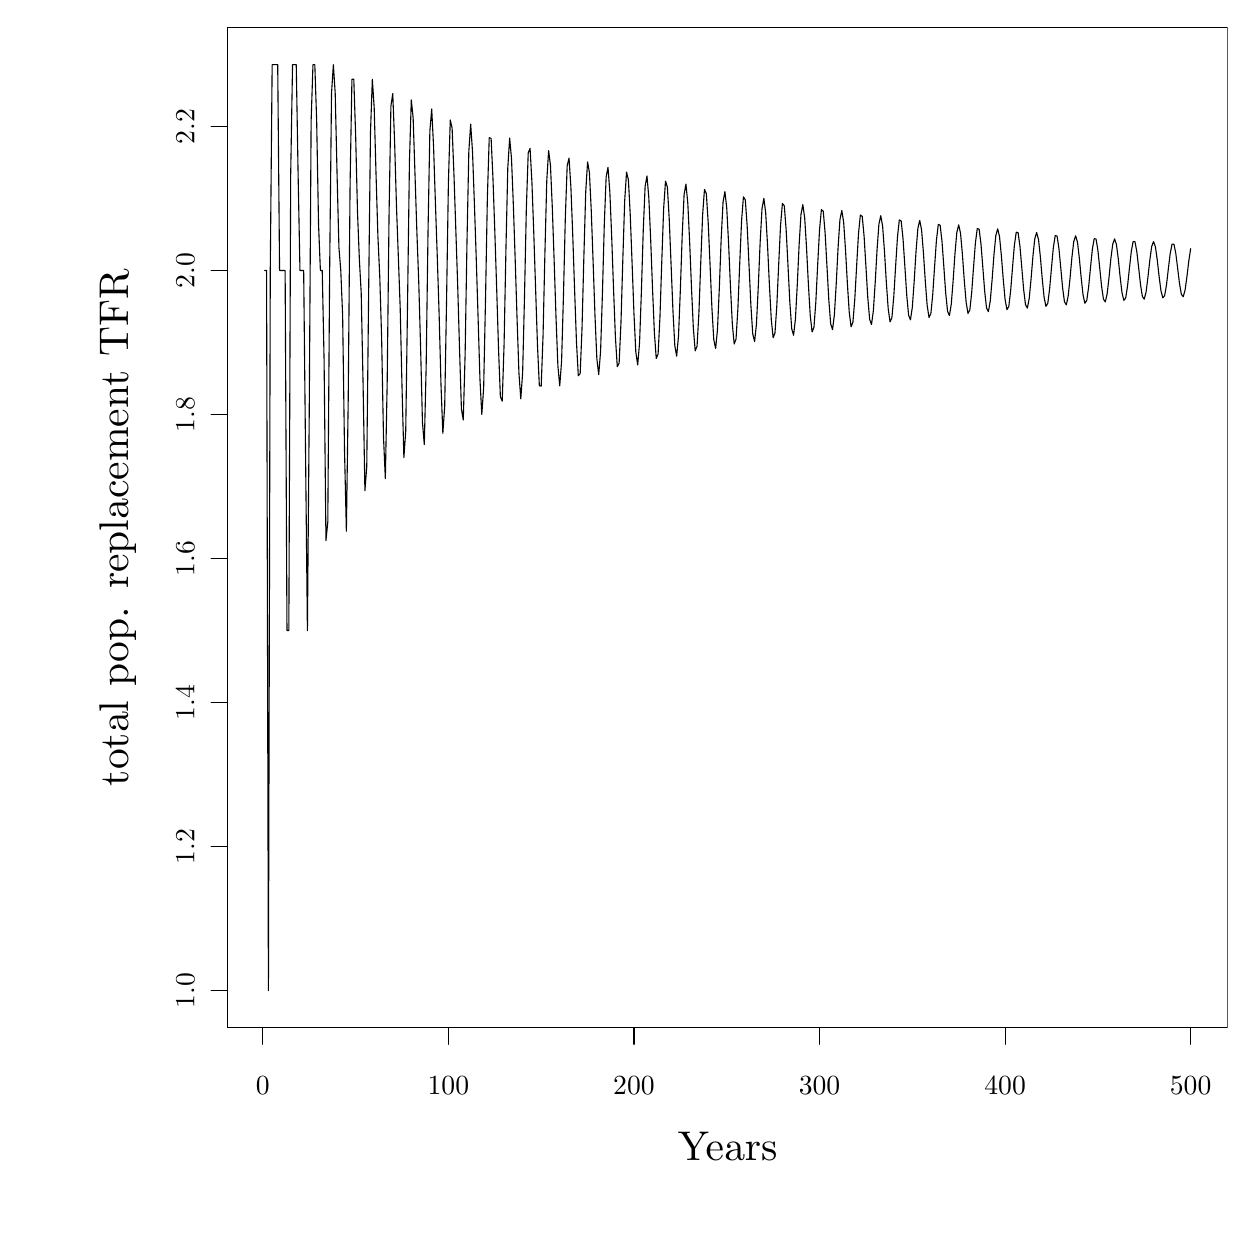
\begin{tikzpicture}[x=1pt,y=1pt]
\definecolor[named]{drawColor}{rgb}{0.00,0.00,0.00}
\definecolor[named]{fillColor}{rgb}{1.00,1.00,1.00}
\fill[color=fillColor,] (0,0) rectangle (433.62,433.62);
\begin{scope}
\path[clip] ( 72.27, 72.27) rectangle (433.62,433.62);
\definecolor[named]{drawColor}{rgb}{0.16,0.82,0.37}
\definecolor[named]{drawColor}{rgb}{0.00,0.00,0.00}

\draw[color=drawColor,line cap=round,line join=round,fill opacity=0.00,] ( 85.65,345.88) --
	( 86.32,345.88) --
	( 86.99, 85.65) --
	( 87.66,345.88) --
	( 88.34,420.24) --
	( 89.01,420.24) --
	( 89.68,420.24) --
	( 90.35,420.24) --
	( 91.02,345.88) --
	( 91.69,345.88) --
	( 92.36,345.88) --
	( 93.03,345.88) --
	( 93.70,215.77) --
	( 94.37,215.77) --
	( 95.04,380.58) --
	( 95.71,420.24) --
	( 96.38,420.24) --
	( 97.05,420.24) --
	( 97.72,380.58) --
	( 98.39,345.88) --
	( 99.06,345.88) --
	( 99.73,345.88) --
	(100.40,280.83) --
	(101.08,215.77) --
	(101.75,295.52) --
	(102.42,399.73) --
	(103.09,420.24) --
	(103.76,420.24) --
	(104.43,399.73) --
	(105.10,362.67) --
	(105.77,345.88) --
	(106.44,345.88) --
	(107.11,313.36) --
	(107.78,248.30) --
	(108.45,255.01) --
	(109.12,345.88) --
	(109.79,409.80) --
	(110.46,420.24) --
	(111.13,409.80) --
	(111.80,380.58) --
	(112.47,354.15) --
	(113.14,345.88) --
	(113.81,329.62) --
	(114.49,280.83) --
	(115.16,251.63) --
	(115.83,299.34) --
	(116.50,377.02) --
	(117.17,414.97) --
	(117.84,414.97) --
	(118.51,394.82) --
	(119.18,367.04) --
	(119.85,349.98) --
	(120.52,337.75) --
	(121.19,305.22) --
	(121.86,266.28) --
	(122.53,275.10) --
	(123.20,337.21) --
	(123.87,395.67) --
	(124.54,414.97) --
	(125.21,404.72) --
	(125.88,380.58) --
	(126.55,358.38) --
	(127.22,343.84) --
	(127.90,321.49) --
	(128.57,285.79) --
	(129.24,270.65) --
	(129.91,305.52) --
	(130.58,365.82) --
	(131.25,405.24) --
	(131.92,409.80) --
	(132.59,392.39) --
	(133.26,369.25) --
	(133.93,351.04) --
	(134.60,332.64) --
	(135.27,303.66) --
	(135.94,278.27) --
	(136.61,287.82) --
	(137.28,335.04) --
	(137.95,385.23) --
	(138.62,407.52) --
	(139.29,400.97) --
	(139.96,380.58) --
	(140.63,360.01) --
	(141.31,341.79) --
	(141.98,318.14) --
	(142.65,291.01) --
	(143.32,282.99) --
	(143.99,311.01) --
	(144.66,359.68) --
	(145.33,396.29) --
	(146.00,404.22) --
	(146.67,390.59) --
	(147.34,370.11) --
	(148.01,350.80) --
	(148.68,329.93) --
	(149.35,304.59) --
	(150.02,287.03) --
	(150.69,296.80) --
	(151.36,334.91) --
	(152.03,377.75) --
	(152.70,400.25) --
	(153.37,397.32) --
	(154.05,380.17) --
	(154.72,360.32) --
	(155.39,340.29) --
	(156.06,317.25) --
	(156.73,295.85) --
	(157.40,291.86) --
	(158.07,315.55) --
	(158.74,356.00) --
	(159.41,388.93) --
	(160.08,398.78) --
	(160.75,388.61) --
	(161.42,370.08) --
	(162.09,350.20) --
	(162.76,328.73) --
	(163.43,306.57) --
	(164.10,293.87) --
	(164.77,303.55) --
	(165.44,335.46) --
	(166.11,372.28) --
	(166.78,393.85) --
	(167.46,393.64) --
	(168.13,379.20) --
	(168.80,360.01) --
	(169.47,339.39) --
	(170.14,317.64) --
	(170.81,300.25) --
	(171.48,298.66) --
	(172.15,319.27) --
	(172.82,353.62) --
	(173.49,383.01) --
	(174.16,393.74) --
	(174.83,386.32) --
	(175.50,369.47) --
	(176.17,349.60) --
	(176.84,328.47) --
	(177.51,308.96) --
	(178.18,299.46) --
	(178.85,308.84) --
	(179.52,336.21) --
	(180.19,368.17) --
	(180.87,388.38) --
	(181.54,390.00) --
	(182.21,377.78) --
	(182.88,359.41) --
	(183.55,338.96) --
	(184.22,318.70) --
	(184.89,304.23) --
	(185.56,304.10) --
	(186.23,322.35) --
	(186.90,352.00) --
	(187.57,378.23) --
	(188.24,389.19) --
	(188.91,383.82) --
	(189.58,368.47) --
	(190.25,349.09) --
	(190.92,328.79) --
	(191.59,311.48) --
	(192.26,304.17) --
	(192.93,313.12) --
	(193.61,336.99) --
	(194.28,365.01) --
	(194.95,383.71) --
	(195.62,386.48) --
	(196.29,376.05) --
	(196.96,358.67) --
	(197.63,338.87) --
	(198.30,320.12) --
	(198.97,307.84) --
	(199.64,308.60) --
	(200.31,324.91) --
	(200.98,350.85) --
	(201.65,374.32) --
	(202.32,385.10) --
	(202.99,381.21) --
	(203.66,367.26) --
	(204.33,348.68) --
	(205.00,329.46) --
	(205.67,313.99) --
	(206.34,308.22) --
	(207.02,316.67) --
	(207.69,337.74) --
	(208.36,362.50) --
	(209.03,379.71) --
	(209.70,383.14) --
	(210.37,374.16) --
	(211.04,357.87) --
	(211.71,339.00) --
	(212.38,321.71) --
	(213.05,311.12) --
	(213.72,312.41) --
	(214.39,327.09) --
	(215.06,350.00) --
	(215.73,371.07) --
	(216.40,381.43) --
	(217.07,378.61) --
	(217.74,365.93) --
	(218.41,348.36) --
	(219.08,330.33) --
	(219.75,316.42) --
	(220.43,311.76) --
	(221.10,319.68) --
	(221.77,338.43) --
	(222.44,360.47) --
	(223.11,376.25) --
	(223.78,380.01) --
	(224.45,372.20) --
	(225.12,357.06) --
	(225.79,339.29) --
	(226.46,323.37) --
	(227.13,314.10) --
	(227.80,315.69) --
	(228.47,328.96) --
	(229.14,349.36) --
	(229.81,368.34) --
	(230.48,378.14) --
	(231.15,376.07) --
	(231.82,364.56) --
	(232.49,348.10) --
	(233.17,331.30) --
	(233.84,318.74) --
	(234.51,314.89) --
	(235.18,322.26) --
	(235.85,339.07) --
	(236.52,358.79) --
	(237.19,373.24) --
	(237.86,377.10) --
	(238.53,370.26) --
	(239.20,356.26) --
	(239.87,339.65) --
	(240.54,325.01) --
	(241.21,316.82) --
	(241.88,318.55) --
	(242.55,330.59) --
	(243.22,348.86) --
	(243.89,365.99) --
	(244.56,375.17) --
	(245.23,373.66) --
	(245.90,363.20) --
	(246.58,347.89) --
	(247.25,332.31) --
	(247.92,320.92) --
	(248.59,317.68) --
	(249.26,324.52) --
	(249.93,339.65) --
	(250.60,357.38) --
	(251.27,370.58) --
	(251.94,374.41) --
	(252.61,368.38) --
	(253.28,355.48) --
	(253.95,340.06) --
	(254.62,326.61) --
	(255.29,319.31) --
	(255.96,321.08) --
	(256.63,332.02) --
	(257.30,348.45) --
	(257.97,363.96) --
	(258.64,372.50) --
	(259.31,371.38) --
	(259.99,361.88) --
	(260.66,347.72) --
	(261.33,333.31) --
	(262.00,322.96) --
	(262.67,320.19) --
	(263.34,326.51) --
	(264.01,340.18) --
	(264.68,356.17) --
	(265.35,368.23) --
	(266.02,371.94) --
	(266.69,366.59) --
	(267.36,354.75) --
	(268.03,340.48) --
	(268.70,328.13) --
	(269.37,321.58) --
	(270.04,323.33) --
	(270.71,333.29) --
	(271.38,348.13) --
	(272.05,362.19) --
	(272.72,370.09) --
	(273.40,369.25) --
	(274.07,360.63) --
	(274.74,347.57) --
	(275.41,334.29) --
	(276.08,324.86) --
	(276.75,322.45) --
	(277.42,328.27) --
	(278.09,340.66) --
	(278.76,355.13) --
	(279.43,366.14) --
	(280.10,369.67) --
	(280.77,364.91) --
	(281.44,354.05) --
	(282.11,340.90) --
	(282.78,329.57) --
	(283.45,323.66) --
	(284.12,325.34) --
	(284.79,334.42) --
	(285.46,347.85) --
	(286.14,360.62) --
	(286.81,367.91) --
	(287.48,367.28) --
	(288.15,359.44) --
	(288.82,347.44) --
	(289.49,335.22) --
	(290.16,326.61) --
	(290.83,324.50) --
	(291.50,329.85) --
	(292.17,341.10) --
	(292.84,354.21) --
	(293.51,364.26) --
	(294.18,367.59) --
	(294.85,363.34) --
	(295.52,353.40) --
	(296.19,341.30) --
	(296.86,330.91) --
	(297.53,325.56) --
	(298.20,327.16) --
	(298.87,335.44) --
	(299.55,347.62) --
	(300.22,359.23) --
	(300.89,365.93) --
	(301.56,365.45) --
	(302.23,358.34) --
	(302.90,347.32) --
	(303.57,336.09) --
	(304.24,328.24) --
	(304.91,326.36) --
	(305.58,331.28) --
	(306.25,341.50) --
	(306.92,353.40) --
	(307.59,362.58) --
	(308.26,365.69) --
	(308.93,361.88) --
	(309.60,352.80) --
	(310.27,341.68) --
	(310.94,332.16) --
	(311.61,327.30) --
	(312.28,328.80) --
	(312.96,336.36) --
	(313.63,347.42) --
	(314.30,357.98) --
	(314.97,364.14) --
	(315.64,363.77) --
	(316.31,357.31) --
	(316.98,347.21) --
	(317.65,336.91) --
	(318.32,329.73) --
	(318.99,328.05) --
	(319.66,332.56) --
	(320.33,341.86) --
	(321.00,352.69) --
	(321.67,361.06) --
	(322.34,363.96) --
	(323.01,360.53) --
	(323.68,352.24) --
	(324.35,342.05) --
	(325.02,333.32) --
	(325.70,328.89) --
	(326.37,330.29) --
	(327.04,337.19) --
	(327.71,347.25) --
	(328.38,356.87) --
	(329.05,362.51) --
	(329.72,362.23) --
	(330.39,356.36) --
	(331.06,347.12) --
	(331.73,337.67) --
	(332.40,331.11) --
	(333.07,329.59) --
	(333.74,333.72) --
	(334.41,342.20) --
	(335.08,352.05) --
	(335.75,359.69) --
	(336.42,362.37) --
	(337.09,359.28) --
	(337.76,351.72) --
	(338.43,342.38) --
	(339.11,334.39) --
	(339.78,330.35) --
	(340.45,331.65) --
	(341.12,337.94) --
	(341.79,347.10) --
	(342.46,355.86) --
	(343.13,361.03) --
	(343.80,360.82) --
	(344.47,355.48) --
	(345.14,347.03) --
	(345.81,338.38) --
	(346.48,332.37) --
	(347.15,331.00) --
	(347.82,334.78) --
	(348.49,342.50) --
	(349.16,351.47) --
	(349.83,358.45) --
	(350.50,360.93) --
	(351.17,358.14) --
	(351.84,351.24) --
	(352.52,342.69) --
	(353.19,335.37) --
	(353.86,331.69) --
	(354.53,332.88) --
	(355.20,338.62) --
	(355.87,346.97) --
	(356.54,354.95) --
	(357.21,359.69) --
	(357.88,359.53) --
	(358.55,354.67) --
	(359.22,346.95) --
	(359.89,339.02) --
	(360.56,333.53) --
	(361.23,332.28) --
	(361.90,335.74) --
	(362.57,342.78) --
	(363.24,350.95) --
	(363.91,357.32) --
	(364.58,359.61) --
	(365.26,357.09) --
	(365.93,350.80) --
	(366.60,342.98) --
	(367.27,336.27) --
	(367.94,332.91) --
	(368.61,334.01) --
	(369.28,339.25) --
	(369.95,346.85) --
	(370.62,354.13) --
	(371.29,358.47) --
	(371.96,358.35) --
	(372.63,353.93) --
	(373.30,346.87) --
	(373.97,339.62) --
	(374.64,334.59) --
	(375.31,333.45) --
	(375.98,336.62) --
	(376.65,343.04) --
	(377.32,350.48) --
	(377.99,356.30) --
	(378.67,358.41) --
	(379.34,356.13) --
	(380.01,350.39) --
	(380.68,343.24) --
	(381.35,337.10) --
	(382.02,334.02) --
	(382.69,335.03) --
	(383.36,339.81) --
	(384.03,346.75) --
	(384.70,353.39) --
	(385.37,357.35) --
	(386.04,357.27) --
	(386.71,353.25) --
	(387.38,346.80) --
	(388.05,340.17) --
	(388.72,335.56) --
	(389.39,334.53) --
	(390.06,337.41) --
	(390.73,343.27) --
	(391.40,350.06) --
	(392.08,355.37) --
	(392.75,357.31) --
	(393.42,355.25) --
	(394.09,350.02) --
	(394.76,343.48) --
	(395.43,337.86) --
	(396.10,335.05) --
	(396.77,335.97) --
	(397.44,340.33) --
	(398.11,346.66) --
	(398.78,352.71) --
	(399.45,356.34) --
	(400.12,356.28) --
	(400.79,352.63) --
	(401.46,346.74) --
	(402.13,340.67) --
	(402.80,336.46) --
	(403.47,335.51) --
	(404.14,338.14) --
	(404.81,343.49) --
	(405.49,349.68) --
	(406.16,354.53) --
	(406.83,356.31) --
	(407.50,354.45) --
	(408.17,349.67) --
	(408.84,343.70) --
	(409.51,338.56) --
	(410.18,335.98) --
	(410.85,336.82) --
	(411.52,340.81) --
	(412.19,346.58) --
	(412.86,352.10) --
	(413.53,355.42) --
	(414.20,355.38) --
	(414.87,352.05) --
	(415.54,346.68) --
	(416.21,341.12) --
	(416.88,337.27) --
	(417.55,336.40) --
	(418.23,338.81) --
	(418.90,343.68) --
	(419.57,349.33) --
	(420.24,353.76);
\end{scope}
\begin{scope}
\path[clip] (  0.00,  0.00) rectangle (433.62,433.62);
\definecolor[named]{drawColor}{rgb}{0.16,0.82,0.37}
\definecolor[named]{drawColor}{rgb}{0.00,0.00,0.00}

\draw[color=drawColor,line cap=round,line join=round,fill opacity=0.00,] ( 84.98, 72.27) -- (420.24, 72.27);

\draw[color=drawColor,line cap=round,line join=round,fill opacity=0.00,] ( 84.98, 72.27) -- ( 84.98, 66.27);

\draw[color=drawColor,line cap=round,line join=round,fill opacity=0.00,] (152.03, 72.27) -- (152.03, 66.27);

\draw[color=drawColor,line cap=round,line join=round,fill opacity=0.00,] (219.08, 72.27) -- (219.08, 66.27);

\draw[color=drawColor,line cap=round,line join=round,fill opacity=0.00,] (286.14, 72.27) -- (286.14, 66.27);

\draw[color=drawColor,line cap=round,line join=round,fill opacity=0.00,] (353.19, 72.27) -- (353.19, 66.27);

\draw[color=drawColor,line cap=round,line join=round,fill opacity=0.00,] (420.24, 72.27) -- (420.24, 66.27);

\node[color=drawColor,anchor=base,inner sep=0pt, outer sep=0pt, scale=  1.00] at ( 84.98, 48.27) {0%
};

\node[color=drawColor,anchor=base,inner sep=0pt, outer sep=0pt, scale=  1.00] at (152.03, 48.27) {100%
};

\node[color=drawColor,anchor=base,inner sep=0pt, outer sep=0pt, scale=  1.00] at (219.08, 48.27) {200%
};

\node[color=drawColor,anchor=base,inner sep=0pt, outer sep=0pt, scale=  1.00] at (286.14, 48.27) {300%
};

\node[color=drawColor,anchor=base,inner sep=0pt, outer sep=0pt, scale=  1.00] at (353.19, 48.27) {400%
};

\node[color=drawColor,anchor=base,inner sep=0pt, outer sep=0pt, scale=  1.00] at (420.24, 48.27) {500%
};

\draw[color=drawColor,line cap=round,line join=round,fill opacity=0.00,] ( 72.27, 85.65) -- ( 72.27,397.93);

\draw[color=drawColor,line cap=round,line join=round,fill opacity=0.00,] ( 72.27, 85.65) -- ( 66.27, 85.65);

\draw[color=drawColor,line cap=round,line join=round,fill opacity=0.00,] ( 72.27,137.70) -- ( 66.27,137.70);

\draw[color=drawColor,line cap=round,line join=round,fill opacity=0.00,] ( 72.27,189.75) -- ( 66.27,189.75);

\draw[color=drawColor,line cap=round,line join=round,fill opacity=0.00,] ( 72.27,241.79) -- ( 66.27,241.79);

\draw[color=drawColor,line cap=round,line join=round,fill opacity=0.00,] ( 72.27,293.84) -- ( 66.27,293.84);

\draw[color=drawColor,line cap=round,line join=round,fill opacity=0.00,] ( 72.27,345.88) -- ( 66.27,345.88);

\draw[color=drawColor,line cap=round,line join=round,fill opacity=0.00,] ( 72.27,397.93) -- ( 66.27,397.93);

\node[rotate= 90.00,color=drawColor,anchor=base,inner sep=0pt, outer sep=0pt, scale=  1.00] at ( 60.27, 85.65) {1.0%
};

\node[rotate= 90.00,color=drawColor,anchor=base,inner sep=0pt, outer sep=0pt, scale=  1.00] at ( 60.27,137.70) {1.2%
};

\node[rotate= 90.00,color=drawColor,anchor=base,inner sep=0pt, outer sep=0pt, scale=  1.00] at ( 60.27,189.75) {1.4%
};

\node[rotate= 90.00,color=drawColor,anchor=base,inner sep=0pt, outer sep=0pt, scale=  1.00] at ( 60.27,241.79) {1.6%
};

\node[rotate= 90.00,color=drawColor,anchor=base,inner sep=0pt, outer sep=0pt, scale=  1.00] at ( 60.27,293.84) {1.8%
};

\node[rotate= 90.00,color=drawColor,anchor=base,inner sep=0pt, outer sep=0pt, scale=  1.00] at ( 60.27,345.88) {2.0%
};

\node[rotate= 90.00,color=drawColor,anchor=base,inner sep=0pt, outer sep=0pt, scale=  1.00] at ( 60.27,397.93) {2.2%
};

\draw[color=drawColor,line cap=round,line join=round,fill opacity=0.00,] ( 72.27, 72.27) --
	(433.62, 72.27) --
	(433.62,433.62) --
	( 72.27,433.62) --
	( 72.27, 72.27);
\end{scope}
\begin{scope}
\path[clip] (  0.00,  0.00) rectangle (433.62,433.62);
\definecolor[named]{drawColor}{rgb}{0.16,0.82,0.37}
\definecolor[named]{drawColor}{rgb}{0.00,0.00,0.00}

\node[color=drawColor,anchor=base,inner sep=0pt, outer sep=0pt, scale=  1.50] at (252.95, 24.27) {Years%
};

\node[rotate= 90.00,color=drawColor,anchor=base,inner sep=0pt, outer sep=0pt, scale=  1.50] at ( 36.27,252.95) {total pop. replacement TFR%
};
\end{scope}
\end{tikzpicture}

}
\end{center}
\caption{TFR necessary to maintain population at 200, given a sudden 0.5 increase in lifespan, projected 500 years.}
\label{fig:one}
\end{figure}

Under the conditions we specified, the TFR, calculated in the usual way, would need to adjust from year to year in order to keep the total population steady at 200. The time series, projected 500 years forward, obtains a sinusoidal pattern, with exponentially decreasing amplitude and a constant period of 11 years. 1000 years forward in time, there is still year to year variation in TFR necessary, although the range from trough to peak is a mere 0.009 births, barely noticeable. Since this scenario takes so long to converge, we call it weakly ergodic. Real human populations, with many age classes and clear age patterns to demographic functions, tend to converge much faster. So it is that populations lose their memory of ruptures in the distant past, the blending of behavior over ages dampens the impact of shocks, such as a sudden increase in life expectancy.

We note that in both scenarios TFR attains a value of 2, in the first case (the typical case) immediately, in the second case (that of Dr. Cabr\'{e}) asymptotically. In the first case the population grows, and in the second case it remains steady, with the size of each generation decreasing by a small amount in order to make room for the surviving elderly. In the first case, reproducing men and women experience no shocks, and in the second they must adjust according to the present population size and structure. As a matter of course, the cohort TFR in the latter case will also have a sinusoidal shape, with some generations having increasing fertility over their reproductive careers, others decreasing, other peaking, others bottoming out, in each case according to the demands of the replacement TFR condition in the present year. Certainly, the first scenario is not nearly as smooth as its constant TFR would suggest, for there must be ripple effects in the intergenerational care transfers implied by increased survival of the elderly, a consideration that beyond our scope.

The present discourse provides no criterion by which to judge one or the other scenario more or less desirable, but we conclude that both are indeed consistent visions. Similarly, we could simulate more complex and realistic pictures, where fertility and mortality display age patterns, and these determine the stationary age structure in year 0. Mortality decreases have tended to be gradual and sustained in recent decades, and we could model it this way too. So too could we alter the modeled sex ratio at birth and pre-reproductive mortality, and optimize TFR to hold the population constant. In doing so, we would notice that the TFR required for generational stability is mutable with changes in the sex ratio at birth and in infant and youth mortality, but it is not mutable with changes in post-reproductive mortality. The condition of total population stability, however, would entail replacement TFR adjustments due to any change in the sex ratio at birth or mortality. 

		\subsubsection{Response to imbalances in the stocks of the sexes}

Again with the case of 10 ages, imagine now that instead of a 1:1 sex ratio at birth, that it changes to something rather drastic, like 2:1, i.e. 2 males for each female. Assume also that there is no excess male mortality, and that males later in life do not migrate away in frustration. What would be required for us to maintain 1) stability of the generations and 2) stability of the total population?

In the first case 1.a), we begin with equal stocks of males and females in reproductive ages, the new generations are still 20 total births, but they are divided into 6.67 girls to 13.33 boys. When these generations, still liberated from early-life mortality, come of reproductive age, the stocks of available women will be lower than was the case before. In order to maintain generation size, women must increase their fertility. Some males of reproductive age will never mate, especially if the society practices strict monogamy. There is much to be said of how pluralities of humans adjust to imbalances in the sex ratio among members of reproductive age, and this topic will be treated later on in a different section. For the time being, we focus just on the arithmetic implied by meeting both conditions of stability. When the first sex-imbalanced generation arrives to age 2 (the first reproductive age), these 6.67 women are added to another 30 from the prior balanced generations. 36.67 women are then called to duty to produce 20 births. In the next year 33.33 women must produce 20 births, followed by 30 women, and finally by 26.67 women. From then on, there will be a steady 26.67 women available to produce 20 births, entailing a sharp increase in TFR:

\begin{align}
TFR = \sum_{a=2}^{5} \frac{B_a}{F_a} = 4 \times\frac{5}{6.67} = 3 
\end{align}

This increase will happen in even steps over a 4 year period, starting when the first imbalanced generation reaches reproductive age. Of the males, we notice no change at first, then an additional 3.33 males each year for four years. This entails a linear fall in male fertility: 20 births are first produced by 40, then 43.33, 46.66, 50 and finally 53.33 males, and so it remains for the rest of time, with male TFR at a steady 1.5, disappointingly lower than when there were parity sex ratios at birth. Free of increases in life expectancy, the population remains the same size.

This scenario diverges from the usual expectation of generation replacement in the following way: Here we have replaced the entire mixed-sex generation, while typically population biologists require us to fully replace a \textit{generation of females}. This is so because it is the females that are asked to increase their fertility, and clearly they would be the limiting factor in this experiment. 

How would this scenario 1.b) change in order to meet the population biologist?s request? If the change in sex ratio at birth is sudden, changes would have to happen in the very first year, and they would not be gradual. In the first year, rather than 1:1, we have 2:1 males to females: Women must immediately increase their fertility by 50\% in order to hold the number of girls born to 10, entailing 30 births, and an immediate TFR of 3, from then on steady. At first, men too must increase their fertility by 50\% in order to adjust for the shock; it jumps to 3. When the first sex imbalanced generations come of reproductive age, the denominators of male TFR begin to inflate, 30 births are fathered from 40 then 43.33, 46.66, 50 and finally stabilizing at 53.33 males. Male TFR then falls in a linear fashion over four years to a value of 2.25 ($4\times\frac{30}{53.33}$). The total population increases by 10 male individuals per year for 10 years, then holds steady at 300. The population biologist tells us that in order to maintain a population, we must maintain its females, and in order to do so in the event of an increase in the sex ratio at birth, the population increases by a factor proportional to the change in the inverse of the sex ratio at birth (50\% in this case). We notice that both males and females are asked to increase their fertility in this case, all the more surprising since there are now relatively more males than before. Let us hope that this island of humans is able to cope with its increased population, for this scenario follows demographic wisdom!

Returning to condition 2, that of holding the total population stable, we first note that the response required of women is identical to that of scenario 1.a: As smaller generations of women enter reproductive ages, they must incrementally increase their fertility, until arriving at a TFR of 3. This keeps both the generation size and the total population size steady at 20 and 200, respectively, although the total number of females will decrease to 66.67 and the total number of males will increase to 133.33, as in case 1.a. Males arrive at a TFR of 1.5, as in case 1.a. If we ask that the population maintain the same total count of females, then the solution also falls back to scenario 2.b. Female fertility immediately increases in order to produce enough baby girls, thereby making male fertility also increase; female fertility maintains a steady high level, while male fertility falls linearly from 3 to 2.25, still higher than it was before.

We observe how summary measures of fertility must adjust for these two most basic of biological changes: longer lifespan and changes in the sex ratio at birth. The responses require change in accordance with our optimization of replacement fertility, which itself is a function of our criterion for stability. So it is that stability of population structure and stability of population size are two very different concepts entailing very different replacement thresholds. We note that the stability with which demographers have long engaged is the former, ergodic stability, while critics of cornucopian economics have tended to side with the later a total population held at a limit. 

		\subsubsection{Response to differences in the age combinations and age-ranges of mates}

Take the initial case with 10 individuals of each sex at every age, and imagine now instead of perfect age homogamy, that males and females mate over different age ranges. Females reproduce from age 2 to 5 (4 ages), and males from age 2-7 (6 ages). We ignore age combinations of females and males, and just assume that each age has the same fertility within each sex. In general, nothing changes with respect to our variants of replacement, female TFR is the same and male TFR is the same, both still 2. However, male fertility is now $\frac{1}{3}$ lower in each reproductive age (20 births come from 60 males instead of from 40) while female age-specific fertility remains the same.

One step further, we can randomize parent age-matching between males and females within these ranges (2-5 for females and 2-7 for males), so that births are not evenly distributed. That is to say, births are randomly distributed over age combinations, still summing to 20, but with an uneven distribution of births among males and an uneven distribution among females. The stocks of males and females are still evenly distributed over the ages as before. In this case, it would be possible to calculate a specific fertility rate for each combination of male and female reproductive ages. It still holds here that if there are 20 births, male TFR and female TFR will each be equal to 2, even with random mixing of partners, as long as stocks are evenly distributed as in the example. Furthermore, we can still retrieve a convenient mixed-sex replacement TFR of 1, placing both males and females in the denominator as in the case of equal age ranges and perfect homogamy. To do so, take the birth counts from each potential partner age dyad. Divide each by the sum of males and females from the corresponding ages. The resulting table will still sum to 1 in this example.

To state this observation formally, where $\textbf{B}_{xy}$ is a matrix of birth counts by mothers' age $x$ in rows and fathers' age $y$ in columns. $\textbf{p}_x$ and $\textbf{p}_y$ are count vectors of females and males aged $x$ and $y$ respectively. Then a simple mixed-sex TFR$_{mf}$ might be\footnote{Here the $\otimes$ operator indicates the outer sum, or tensor sum. px and py are vectors, and their outer sum results in a matrix whose row dimension is equal to the length $\textbf{p}_x$ and whose column dimension is equal to the length of $\textbf{p}_y$, and whose elements consist in the element-wise sums of $\textbf{p}_x$ and $\textbf{p}_y$. Division is possible because the matrix dimensions are identical.}:

\begin{align}
TFR_{mf} = \sum\frac{\textbf{B}_{xy}}{\textbf{p}_x \otimes \textbf{p}_y}
\end{align}

Recall that the population pyramid is still uniform in our example, with 10 males and 10 females in each age group. As long as there are a total of 20 births in $\textbf{B}_{xy}$, the replacement TFR$_{mf}$ will be equal to 1.

This observation continues to hold even if we tilt the stocks of males and females evenly toward one or the other sex. For example, instead of 10 in each age class of males and females, we place 9 in each age class of females and 11 in each age class of males. In this case, male and female TFR will indeed differ, but the mixed sex TFR$_{mf}$ will continue to sum to 1, a convenient result. This is because the sum of each age combination of males and females is still 20, as when there are 10 individuals in each age. In this case we have 20 total births and 20 total individuals in each generation, as well as 20 dying in the old. The replacement birth \textit{count} will be 20 no matter which kind of stability we wish to satisfy, despite having 9 females and 11 males in each age, supposing that this ratio also translates over into the sex ratio at birth.

If we change the counts of males and females in each age to, say, 9 females and 12 males, this result will no longer pertain. In this case the above formula will essentially reduce to the ratio $\frac{20}{21}$, a mixed sex TFR a less than 1 (0.952). This is consistent because in this case we will have changed both replacement thresholds- generations of size 21 and 21 population exits: In this case there ought to have been 21 births whether aiming for generational or total population replacement. 

From this we learn that age mixing and different age ranges for males and females are not what complicate the interpretation of common (female) TFR. Differences in stocks between males and females, non-unity sex ratios within or between mating ages, do complicate its interpretation, even when replacement is satisfied. In the case of 9 females in each of 4 ages (to 11 males in each of 6), we observe a TFR of $\frac{20}{4\times9}=2.222$. However, we know that the replacement criterion has been satisfied exactly. Are we to understand that the replacement TFR for females under these circumstances is 2.222, while that for males is $\frac{20}{6\times11}=1.818$? This is inconsistent and confusing. However, the mixed sex TFR$_{mf}$ still yields a value of 1, consistent with the very basic initial scenario.

There are conditions that complicate variants of this scenario further, and they will be treated separately in a pedantic way, so that we may become familiar with the difficulties of the problem at hand.

		\subsubsection{Response to subtle differences in the sex ratios of males and females in reproductive ages}

We have seen that differences between the age-specific stocks of males and females do not modify the replacement threshold of our mixed sex TFR$_mf$ , as long as all of their combinations sum to the replacement birth count, in our example 20, and even in the realistic case where males reproduce until later in life.  This continues to hold even when births are randomly distributed over age combos, an unrealistic condition for sure, but one whose satisfaction guarantees that any age curve of fertility will be acceptable. We now change the stocks of males and females in the following way: Males retain their reproductive age range (2-7), but their stocks are staggered, (9,11,9,11,9,11), averaging 10 still. Female stocks are even at 10. Births still sum to 20, but remain randomly distributed over all 24 age combinations of males and females.

In this case, female TFR is still equal to 2, but due to staggered exposures male TFR will not be equal to 2. The exposures serve to weight the randomly distributed births in the numerator, and since these are now staggered, it is unlikely that male age-specific fertility rates will continue to sum to 2. Nor does mixed-sex TFR$_mf$ equal 1, also due to inconsistent weighting. The average generation size is 20, the average sex ratio at birth is 1, and the average number of people dying each year is 20, but all of these things change from year to year. If we are interested only in immediate period replacement, we will require year to year adjustments, depending on the variant of replacement in effect.

For female replacement of the generations, notice in this strange case that over the 4 reproductive ages females will average their own replacement with 1 girl as long as there are 20 births per year. Indeed, due to year to year variation over the ages, some female cohorts will fall short of, and others will exceed 1 girl, but they will all average 1. If the birth count and sex ratio stagger in such a way as to always produce 10 girls, but sometimes 9 and sometimes 11 males, then a particular year's female generational replacement TFR will never equal 2, because some years will only require 19 births, others 21. Convention calls for averaging out female replacement TFR in this case, to keep things simple: If women in this scenario aim for 2 births over their own lifetime, they will all average out to 1 girl, even if the sex ratio at birth toggles in this way. If in each year they succeed as a group, producing 20 births, randomly spread over female ages, period TFR will appear as a stationary time series with random noise (see Figure~\ref{fig:two}), and a mean value of 2 in the long run. 

Note that merely randomizing the age pattern from year to year is not enough to induce stochasticity in the female period TFR in this case: There must also be staggering of the female generation size in order to irregularly weight the age-specific rates. This is here induced by toggling the sex ratio at birth, a fine but relevant point, if we are to make progress. Male TFR will be bound to the same noise pattern, but with attenuated weights from exposure being spread over 6 ages, and a complementary stagger.

If we return to the notion of total population replacement, we would see the same variation in observed period TFR, but the replacement TFR threshold would always be derived from the 20 annual deaths. Since each generation consists in unequal numbers of males and females that always sum to 20, this replacement criterion will always be met, as a simple matter of definition. Furthermore, replacement TFR will be constant, since the female generations also converge quickly to regular staggering.

In general, we conclude that year to year variation in the sex ratio at birth does not play a determining role in choosing a replacement fertility threshold, but it can induce stochasticity in year to year observed fertility rates if the age pattern of fertility is not constant. This can lead to short term deviance from the stated replacement threshold.

\begin{figure}
\begin{center}
% sim2

% keep figure separate from values generation

{\tikzexternaldisable
% Created by tikzDevice version 0.6.1 on 2011-10-25 19:59:55
% !TEX encoding = UTF-8 Unicode
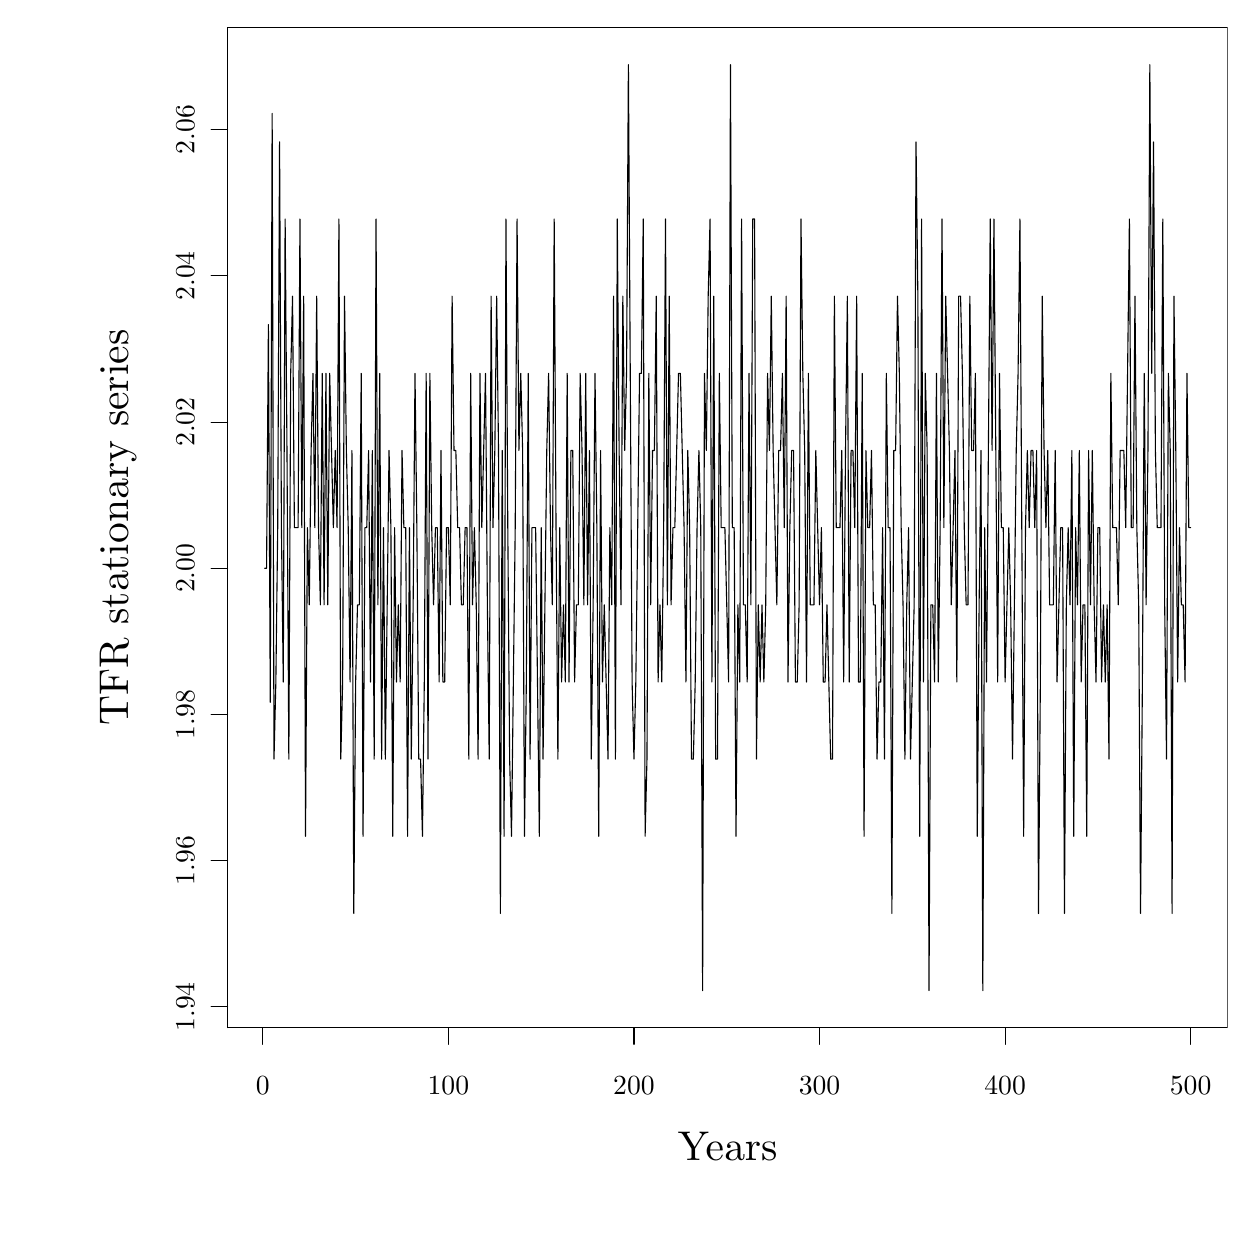
\begin{tikzpicture}[x=1pt,y=1pt]
\definecolor[named]{drawColor}{rgb}{0.00,0.00,0.00}
\definecolor[named]{fillColor}{rgb}{1.00,1.00,1.00}
\fill[color=fillColor,] (0,0) rectangle (433.62,433.62);
\begin{scope}
\path[clip] ( 72.27, 72.27) rectangle (433.62,433.62);
\definecolor[named]{drawColor}{rgb}{0.16,0.82,0.37}
\definecolor[named]{drawColor}{rgb}{0.00,0.00,0.00}

\draw[color=drawColor,line cap=round,line join=round,fill opacity=0.00,] ( 85.65,238.27) --
	( 86.32,238.27) --
	( 86.99,326.32) --
	( 87.66,189.84) --
	( 88.34,402.63) --
	( 89.01,169.30) --
	( 89.68,197.18) --
	( 90.35,252.95) --
	( 91.02,392.35) --
	( 91.69,252.94) --
	( 92.36,197.18) --
	( 93.03,364.47) --
	( 93.70,280.83) --
	( 94.37,169.30) --
	( 95.04,308.71) --
	( 95.71,336.59) --
	( 96.38,252.94) --
	( 97.05,252.94) --
	( 97.72,252.95) --
	( 98.39,364.47) --
	( 99.06,252.95) --
	( 99.73,336.59) --
	(100.40,141.42) --
	(101.08,252.94) --
	(101.75,225.06) --
	(102.42,280.83) --
	(103.09,308.71) --
	(103.76,252.94) --
	(104.43,336.59) --
	(105.10,252.94) --
	(105.77,225.06) --
	(106.44,308.71) --
	(107.11,225.06) --
	(107.78,308.71) --
	(108.45,225.06) --
	(109.12,308.71) --
	(109.79,280.83) --
	(110.46,252.95) --
	(111.13,280.83) --
	(111.80,252.95) --
	(112.47,364.47) --
	(113.14,169.30) --
	(113.81,197.18) --
	(114.49,336.59) --
	(115.16,280.83) --
	(115.83,252.94) --
	(116.50,197.18) --
	(117.17,280.83) --
	(117.84,113.54) --
	(118.51,197.18) --
	(119.18,225.06) --
	(119.85,225.06) --
	(120.52,308.71) --
	(121.19,141.42) --
	(121.86,252.95) --
	(122.53,252.95) --
	(123.20,280.83) --
	(123.87,197.18) --
	(124.54,280.83) --
	(125.21,169.30) --
	(125.88,364.47) --
	(126.55,225.06) --
	(127.22,308.71) --
	(127.90,169.30) --
	(128.57,252.94) --
	(129.24,169.30) --
	(129.91,225.06) --
	(130.58,280.83) --
	(131.25,252.94) --
	(131.92,141.42) --
	(132.59,252.94) --
	(133.26,197.18) --
	(133.93,225.06) --
	(134.60,197.18) --
	(135.27,280.83) --
	(135.94,252.94) --
	(136.61,252.94) --
	(137.28,141.42) --
	(137.95,252.94) --
	(138.62,169.30) --
	(139.29,225.06) --
	(139.96,308.71) --
	(140.63,252.94) --
	(141.31,169.30) --
	(141.98,169.30) --
	(142.65,141.42) --
	(143.32,197.18) --
	(143.99,308.71) --
	(144.66,169.30) --
	(145.33,308.71) --
	(146.00,252.94) --
	(146.67,225.06) --
	(147.34,252.95) --
	(148.01,252.94) --
	(148.68,197.18) --
	(149.35,280.83) --
	(150.02,197.18) --
	(150.69,197.18) --
	(151.36,252.94) --
	(152.03,252.94) --
	(152.70,225.06) --
	(153.37,336.59) --
	(154.05,280.83) --
	(154.72,280.83) --
	(155.39,252.95) --
	(156.06,252.95) --
	(156.73,225.06) --
	(157.40,225.06) --
	(158.07,252.94) --
	(158.74,252.94) --
	(159.41,169.30) --
	(160.08,308.71) --
	(160.75,225.06) --
	(161.42,252.94) --
	(162.09,225.06) --
	(162.76,169.30) --
	(163.43,308.71) --
	(164.10,252.94) --
	(164.77,280.83) --
	(165.44,308.71) --
	(166.11,225.06) --
	(166.78,169.30) --
	(167.46,336.59) --
	(168.13,252.94) --
	(168.80,280.83) --
	(169.47,336.59) --
	(170.14,280.83) --
	(170.81,113.54) --
	(171.48,280.83) --
	(172.15,141.42) --
	(172.82,364.47) --
	(173.49,252.94) --
	(174.16,169.30) --
	(174.83,141.42) --
	(175.50,197.18) --
	(176.17,252.94) --
	(176.84,364.47) --
	(177.51,280.83) --
	(178.18,308.71) --
	(178.85,280.83) --
	(179.52,141.42) --
	(180.19,197.18) --
	(180.87,308.71) --
	(181.54,169.30) --
	(182.21,252.94) --
	(182.88,252.95) --
	(183.55,252.95) --
	(184.22,197.18) --
	(184.89,141.42) --
	(185.56,252.94) --
	(186.23,169.30) --
	(186.90,225.06) --
	(187.57,280.83) --
	(188.24,308.71) --
	(188.91,252.95) --
	(189.58,225.06) --
	(190.25,364.47) --
	(190.92,252.94) --
	(191.59,169.30) --
	(192.26,252.95) --
	(192.93,197.18) --
	(193.61,225.06) --
	(194.28,197.18) --
	(194.95,308.71) --
	(195.62,197.18) --
	(196.29,280.83) --
	(196.96,280.83) --
	(197.63,197.18) --
	(198.30,225.06) --
	(198.97,225.06) --
	(199.64,308.71) --
	(200.31,280.83) --
	(200.98,225.06) --
	(201.65,308.71) --
	(202.32,225.06) --
	(202.99,280.83) --
	(203.66,169.30) --
	(204.33,225.06) --
	(205.00,308.71) --
	(205.67,252.95) --
	(206.34,141.42) --
	(207.02,280.83) --
	(207.69,197.18) --
	(208.36,225.06) --
	(209.03,197.18) --
	(209.70,169.30) --
	(210.37,252.94) --
	(211.04,225.06) --
	(211.71,336.59) --
	(212.38,169.30) --
	(213.05,364.47) --
	(213.72,280.83) --
	(214.39,225.06) --
	(215.06,336.59) --
	(215.73,280.83) --
	(216.40,308.71) --
	(217.07,420.24) --
	(217.74,308.71) --
	(218.41,197.18) --
	(219.08,169.30) --
	(219.75,197.18) --
	(220.43,252.95) --
	(221.10,308.71) --
	(221.77,308.71) --
	(222.44,364.47) --
	(223.11,141.42) --
	(223.78,169.30) --
	(224.45,308.71) --
	(225.12,225.06) --
	(225.79,280.83) --
	(226.46,280.83) --
	(227.13,336.59) --
	(227.80,197.18) --
	(228.47,225.06) --
	(229.14,197.18) --
	(229.81,252.94) --
	(230.48,364.47) --
	(231.15,225.06) --
	(231.82,336.59) --
	(232.49,225.06) --
	(233.17,252.95) --
	(233.84,252.94) --
	(234.51,280.83) --
	(235.18,308.71) --
	(235.85,308.71) --
	(236.52,280.83) --
	(237.19,252.94) --
	(237.86,197.18) --
	(238.53,280.83) --
	(239.20,252.94) --
	(239.87,169.30) --
	(240.54,169.30) --
	(241.21,197.18) --
	(241.88,252.95) --
	(242.55,280.83) --
	(243.22,252.94) --
	(243.89, 85.65) --
	(244.56,308.71) --
	(245.23,280.83) --
	(245.90,336.59) --
	(246.58,364.47) --
	(247.25,197.18) --
	(247.92,336.59) --
	(248.59,169.30) --
	(249.26,169.30) --
	(249.93,308.71) --
	(250.60,252.95) --
	(251.27,252.94) --
	(251.94,252.94) --
	(252.61,225.06) --
	(253.28,197.18) --
	(253.95,420.24) --
	(254.62,252.94) --
	(255.29,252.94) --
	(255.96,141.42) --
	(256.63,225.06) --
	(257.30,197.18) --
	(257.97,364.47) --
	(258.64,225.06) --
	(259.31,225.06) --
	(259.99,197.18) --
	(260.66,308.71) --
	(261.33,225.06) --
	(262.00,364.47) --
	(262.67,364.47) --
	(263.34,169.30) --
	(264.01,225.06) --
	(264.68,197.18) --
	(265.35,225.06) --
	(266.02,197.18) --
	(266.69,225.06) --
	(267.36,308.71) --
	(268.03,280.83) --
	(268.70,336.59) --
	(269.37,280.83) --
	(270.04,252.94) --
	(270.71,225.06) --
	(271.38,280.83) --
	(272.05,280.83) --
	(272.72,308.71) --
	(273.40,252.94) --
	(274.07,336.59) --
	(274.74,197.18) --
	(275.41,252.94) --
	(276.08,280.83) --
	(276.75,280.83) --
	(277.42,197.18) --
	(278.09,197.18) --
	(278.76,225.06) --
	(279.43,364.47) --
	(280.10,308.71) --
	(280.77,280.83) --
	(281.44,197.18) --
	(282.11,308.71) --
	(282.78,225.06) --
	(283.45,225.06) --
	(284.12,225.06) --
	(284.79,280.83) --
	(285.46,252.94) --
	(286.14,225.06) --
	(286.81,252.95) --
	(287.48,197.18) --
	(288.15,197.18) --
	(288.82,225.06) --
	(289.49,197.18) --
	(290.16,169.30) --
	(290.83,169.30) --
	(291.50,336.59) --
	(292.17,252.94) --
	(292.84,252.94) --
	(293.51,252.95) --
	(294.18,280.83) --
	(294.85,197.18) --
	(295.52,280.83) --
	(296.19,336.59) --
	(296.86,197.18) --
	(297.53,280.83) --
	(298.20,280.83) --
	(298.87,252.94) --
	(299.55,336.59) --
	(300.22,197.18) --
	(300.89,197.18) --
	(301.56,308.71) --
	(302.23,141.42) --
	(302.90,280.83) --
	(303.57,252.94) --
	(304.24,252.94) --
	(304.91,280.83) --
	(305.58,225.06) --
	(306.25,225.06) --
	(306.92,169.30) --
	(307.59,197.18) --
	(308.26,197.18) --
	(308.93,252.94) --
	(309.60,169.30) --
	(310.27,308.71) --
	(310.94,252.94) --
	(311.61,252.94) --
	(312.28,113.54) --
	(312.96,280.83) --
	(313.63,280.83) --
	(314.30,336.59) --
	(314.97,308.71) --
	(315.64,252.94) --
	(316.31,225.06) --
	(316.98,169.30) --
	(317.65,225.06) --
	(318.32,252.94) --
	(318.99,169.30) --
	(319.66,197.18) --
	(320.33,225.06) --
	(321.00,392.35) --
	(321.67,336.59) --
	(322.34,141.42) --
	(323.01,364.47) --
	(323.68,197.18) --
	(324.35,308.71) --
	(325.02,280.83) --
	(325.70, 85.65) --
	(326.37,225.06) --
	(327.04,225.06) --
	(327.71,197.18) --
	(328.38,308.71) --
	(329.05,197.18) --
	(329.72,252.95) --
	(330.39,364.47) --
	(331.06,252.94) --
	(331.73,336.59) --
	(332.40,308.71) --
	(333.07,280.83) --
	(333.74,225.06) --
	(334.41,252.94) --
	(335.08,280.83) --
	(335.75,197.18) --
	(336.42,336.59) --
	(337.09,336.59) --
	(337.76,308.71) --
	(338.43,252.94) --
	(339.11,225.06) --
	(339.78,225.06) --
	(340.45,336.59) --
	(341.12,280.83) --
	(341.79,280.83) --
	(342.46,308.71) --
	(343.13,141.42) --
	(343.80,225.06) --
	(344.47,280.83) --
	(345.14, 85.65) --
	(345.81,252.95) --
	(346.48,197.18) --
	(347.15,280.83) --
	(347.82,364.47) --
	(348.49,280.83) --
	(349.16,364.47) --
	(349.83,280.83) --
	(350.50,197.18) --
	(351.17,308.71) --
	(351.84,252.94) --
	(352.52,252.95) --
	(353.19,197.18) --
	(353.86,225.06) --
	(354.53,252.94) --
	(355.20,225.06) --
	(355.87,169.30) --
	(356.54,225.06) --
	(357.21,280.83) --
	(357.88,308.71) --
	(358.55,364.47) --
	(359.22,252.95) --
	(359.89,141.42) --
	(360.56,252.94) --
	(361.23,280.83) --
	(361.90,252.94) --
	(362.57,280.83) --
	(363.24,280.83) --
	(363.91,252.94) --
	(364.58,280.83) --
	(365.26,113.54) --
	(365.93,197.18) --
	(366.60,336.59) --
	(367.27,280.83) --
	(367.94,252.94) --
	(368.61,280.83) --
	(369.28,225.06) --
	(369.95,225.06) --
	(370.62,225.06) --
	(371.29,280.83) --
	(371.96,197.18) --
	(372.63,225.06) --
	(373.30,252.94) --
	(373.97,252.94) --
	(374.64,113.54) --
	(375.31,225.06) --
	(375.98,252.94) --
	(376.65,225.06) --
	(377.32,280.83) --
	(377.99,141.42) --
	(378.67,252.94) --
	(379.34,225.06) --
	(380.01,280.83) --
	(380.68,197.18) --
	(381.35,225.06) --
	(382.02,225.06) --
	(382.69,141.42) --
	(383.36,280.83) --
	(384.03,225.06) --
	(384.70,280.83) --
	(385.37,225.06) --
	(386.04,197.18) --
	(386.71,252.94) --
	(387.38,252.94) --
	(388.05,197.18) --
	(388.72,225.06) --
	(389.39,197.18) --
	(390.06,225.06) --
	(390.73,169.30) --
	(391.40,308.71) --
	(392.08,252.94) --
	(392.75,252.94) --
	(393.42,252.95) --
	(394.09,225.06) --
	(394.76,280.83) --
	(395.43,280.83) --
	(396.10,280.83) --
	(396.77,252.95) --
	(397.44,308.71) --
	(398.11,364.47) --
	(398.78,252.94) --
	(399.45,252.94) --
	(400.12,336.59) --
	(400.79,252.95) --
	(401.46,225.06) --
	(402.13,113.54) --
	(402.80,197.18) --
	(403.47,308.71) --
	(404.14,225.06) --
	(404.81,280.83) --
	(405.49,420.24) --
	(406.16,308.71) --
	(406.83,392.35) --
	(407.50,280.83) --
	(408.17,252.94) --
	(408.84,252.94) --
	(409.51,252.95) --
	(410.18,364.47) --
	(410.85,225.06) --
	(411.52,169.30) --
	(412.19,308.71) --
	(412.86,280.83) --
	(413.53,113.54) --
	(414.20,336.59) --
	(414.87,280.83) --
	(415.54,197.18) --
	(416.21,252.94) --
	(416.88,225.06) --
	(417.55,225.06) --
	(418.23,197.18) --
	(418.90,308.71) --
	(419.57,252.95) --
	(420.24,252.95);
\end{scope}
\begin{scope}
\path[clip] (  0.00,  0.00) rectangle (433.62,433.62);
\definecolor[named]{drawColor}{rgb}{0.16,0.82,0.37}
\definecolor[named]{drawColor}{rgb}{0.00,0.00,0.00}

\draw[color=drawColor,line cap=round,line join=round,fill opacity=0.00,] ( 84.98, 72.27) -- (420.24, 72.27);

\draw[color=drawColor,line cap=round,line join=round,fill opacity=0.00,] ( 84.98, 72.27) -- ( 84.98, 66.27);

\draw[color=drawColor,line cap=round,line join=round,fill opacity=0.00,] (152.03, 72.27) -- (152.03, 66.27);

\draw[color=drawColor,line cap=round,line join=round,fill opacity=0.00,] (219.08, 72.27) -- (219.08, 66.27);

\draw[color=drawColor,line cap=round,line join=round,fill opacity=0.00,] (286.14, 72.27) -- (286.14, 66.27);

\draw[color=drawColor,line cap=round,line join=round,fill opacity=0.00,] (353.19, 72.27) -- (353.19, 66.27);

\draw[color=drawColor,line cap=round,line join=round,fill opacity=0.00,] (420.24, 72.27) -- (420.24, 66.27);

\node[color=drawColor,anchor=base,inner sep=0pt, outer sep=0pt, scale=  1.00] at ( 84.98, 48.27) {0%
};

\node[color=drawColor,anchor=base,inner sep=0pt, outer sep=0pt, scale=  1.00] at (152.03, 48.27) {100%
};

\node[color=drawColor,anchor=base,inner sep=0pt, outer sep=0pt, scale=  1.00] at (219.08, 48.27) {200%
};

\node[color=drawColor,anchor=base,inner sep=0pt, outer sep=0pt, scale=  1.00] at (286.14, 48.27) {300%
};

\node[color=drawColor,anchor=base,inner sep=0pt, outer sep=0pt, scale=  1.00] at (353.19, 48.27) {400%
};

\node[color=drawColor,anchor=base,inner sep=0pt, outer sep=0pt, scale=  1.00] at (420.24, 48.27) {500%
};

\draw[color=drawColor,line cap=round,line join=round,fill opacity=0.00,] ( 72.27, 79.78) -- ( 72.27,396.76);

\draw[color=drawColor,line cap=round,line join=round,fill opacity=0.00,] ( 72.27, 79.78) -- ( 66.27, 79.78);

\draw[color=drawColor,line cap=round,line join=round,fill opacity=0.00,] ( 72.27,132.61) -- ( 66.27,132.61);

\draw[color=drawColor,line cap=round,line join=round,fill opacity=0.00,] ( 72.27,185.44) -- ( 66.27,185.44);

\draw[color=drawColor,line cap=round,line join=round,fill opacity=0.00,] ( 72.27,238.27) -- ( 66.27,238.27);

\draw[color=drawColor,line cap=round,line join=round,fill opacity=0.00,] ( 72.27,291.10) -- ( 66.27,291.10);

\draw[color=drawColor,line cap=round,line join=round,fill opacity=0.00,] ( 72.27,343.93) -- ( 66.27,343.93);

\draw[color=drawColor,line cap=round,line join=round,fill opacity=0.00,] ( 72.27,396.76) -- ( 66.27,396.76);

\node[rotate= 90.00,color=drawColor,anchor=base,inner sep=0pt, outer sep=0pt, scale=  1.00] at ( 60.27, 79.78) {1.94%
};

\node[rotate= 90.00,color=drawColor,anchor=base,inner sep=0pt, outer sep=0pt, scale=  1.00] at ( 60.27,132.61) {1.96%
};

\node[rotate= 90.00,color=drawColor,anchor=base,inner sep=0pt, outer sep=0pt, scale=  1.00] at ( 60.27,185.44) {1.98%
};

\node[rotate= 90.00,color=drawColor,anchor=base,inner sep=0pt, outer sep=0pt, scale=  1.00] at ( 60.27,238.27) {2.00%
};

\node[rotate= 90.00,color=drawColor,anchor=base,inner sep=0pt, outer sep=0pt, scale=  1.00] at ( 60.27,291.10) {2.02%
};

\node[rotate= 90.00,color=drawColor,anchor=base,inner sep=0pt, outer sep=0pt, scale=  1.00] at ( 60.27,343.93) {2.04%
};

\node[rotate= 90.00,color=drawColor,anchor=base,inner sep=0pt, outer sep=0pt, scale=  1.00] at ( 60.27,396.76) {2.06%
};

\draw[color=drawColor,line cap=round,line join=round,fill opacity=0.00,] ( 72.27, 72.27) --
	(433.62, 72.27) --
	(433.62,433.62) --
	( 72.27,433.62) --
	( 72.27, 72.27);
\end{scope}
\begin{scope}
\path[clip] (  0.00,  0.00) rectangle (433.62,433.62);
\definecolor[named]{drawColor}{rgb}{0.16,0.82,0.37}
\definecolor[named]{drawColor}{rgb}{0.00,0.00,0.00}

\node[color=drawColor,anchor=base,inner sep=0pt, outer sep=0pt, scale=  1.50] at (252.95, 24.27) {Years%
};

\node[rotate= 90.00,color=drawColor,anchor=base,inner sep=0pt, outer sep=0pt, scale=  1.50] at ( 36.27,252.95) {TFR stationary series%
};
\end{scope}
\end{tikzpicture}

}

\end{center}
\caption{Stochasticity induced in period female TFR due to toggling sex ratio at birth (9/10; 11/10) and randomizing the female age pattern of fertility (4 reproductive ages), constant 20 births, constant 200 population.}
\label{fig:two}
\end{figure}

Here we have a strange situation where we know that the population satisfies the replacement criterion, but appears not to in most years. It is always possible to exactly retrieve the replacement TFR threshold from the randomness present in every year if instead of dividing births in each age by the observed staggered exposures we divide each age's fertility by the observed average exposure, which is always 10 in our example. Equivalently, we can multiply the ratio of observed exposures to mean exposure into the observed ASFR. Summing these will yield the replacement value of two, even if births are randomly allocated over age. Likewise, the mixed-sex TFRmf can be brought back to 1 by designing weights to bring each element of its denominator back to 20. These treatments are not valid procedures when working with real word data, but serve to validate the simple simulations described here. We presume that real world variation in the sex ratio at birth and year to year variation in the age pattern of fertility are much lower than that simulated here, and real world populations have much larger numbers and more ages; all of these factors would combine to lessen the year to year variation in TFR produced in this example.

	\subsection{A fertility indicator for the population as a whole}

The different versions of replacement, those implying generational replacement or total population replacement, and their variants looking only at females or at both sexes together, entail different replacement criteria. The utility of our common synthetic fertility indicators, TFR and NRR (so far not discussed) does not yet stand in question, but their interpretation will depend on the notion of replacement in use. This makes it tedious to judge whether or not a particular observed TFR is high or low. 

The above scenarios consider fertility measures for males and females separately, under a variety of population conditions. The sexes are indeed at times subject to different pressures in order to meet different replacement criteria. I have tended to separate changes from the base scenario in order to shed light upon the kinds of population changes that a good fertility indicator should dampen out or be sensitive to. Other desirable properties of a fertility indicator include that it respect scale and rank in accordance with the definition of replacement on hand. In this way it can be comparable between different populations, and apply as a summary judgment of the fertility of a single population as a whole, both sexes together. There are certain aspects that we prefer it to be sensitive to, such as market effects between the sexes, an endogenous aspect of population that I have not yet tended to. 

	\subsection{Endogeneity in mixed sex population dynamics}

As stated previously, males and females seek mates under certain constraints, the most universal of which is mate availability. Populations propel themselves forward by reproducing, an activity governed by the population's own inner logic and constrained by exogenous factors, for instance the carrying capacity of a given time and place. Individuals within populations consider aspects of the population itself as constraints. Males are constrained by the availability of females, and females are constrained by the availability of males. Without a male, a female cannot reproduce, and vice versa. Humans (and other species) incur costs in searching for mates, and in competing for mates, especially when mates are scarce. Individual males and females may have different and non-compatible selection criteria, leading to negotiation and tradeoffs. Here I do not consider individual choice mechanisms, but will point out some macro consequences of stock imbalances between the sexes that may have consequences on observed fertility.

In measuring the fertility of the moment, there is no straightforward way to extract how rates might have changed if sex ratios and age distributions had been different. In measuring the fertility of the moment, one also tends to ignore what opportunity costs played out in the aggregate, what losses were incurred, in order to successfully mate: Those are aspects for \textit{explainers}, not for \textit{predictors}. Surely, though, behavior patterns can make fertility increase or decrease in predictable ways. Theories from disciplines beyond demography make this link, but there have been few attempts, and little success, at linking these theories back into prediction. 

Concretely, given present and recent past conditions, demographers project fertility and mortality forward confidently for a few years, but with little confidence thereafter. Precisely, it would be of potential utility for projected future fertility rates to not only be a function of the hopes and judgments of the present, but also of the population structure itself, which we know informs fertility. One avenue for continued future research are in age preferences of the sexes, and substitution preferences when constrained by mate availability. 

\section{A Word on Notation}
This document makes use of a particular set of typfaceing conventions for mathematics and programming, which I here document in order that the remainder of the document be easier to read. First, the following font is used to indicate variables used in text: $R_0$, $f_x$, as opposed to $\text{R}_{\text{0}}$ or $\text{f}_{\text{x}}$. Subscripts indicate ages and transitive states, where ${}_x$ or ${}_y$ indicate age, ${}_t$ indicates time. For instance, $f_x$ is often used to indicate ASFR. Superscripts will be used to differentiate males and females, such that $f_x ^m$ is paternal ASFR and $f_x ^f$ is maternal (typical) ASFR. If male and female variables indexed by age appear together in the same statement or formula, ${}_x$ refers to male age, ${}_y$ refers to female age and ${}_{xy}$ indexes each combination of male and female age. Left subscripts are often dropped, but refer to age interval lengths when used, as is typical in demography, e.g., ${}_5f_20$ specifies the fertility rate for the age-range 20-24. Whenever discrete formulas are used, these left subscripts are implied, but often left out to reduce clutter.

Bold faced lower case variables refer to vectors, which in this context means a vector of age-specific values, e.g., exposures, rates, weights, and such. In this sense, $f_x$ and $\bm{f}$ can be understood as representing the same thing, though vectors will frequently be necessary with particular mathematical operations, and they translate more directly to the style of programming code used in this dissertation. Bold faced upper case variables refer to matrices, such as $\bm{M}$, which could be a marriage table expressed in matrix form, or a birth table $\bm{B}$ cross-tabulated by age of mother and age of father.

All programming for this dissertation has been carried out in the R languange \citep{Rcitation}, and has been integrated with the dissertation typesetting using Sweave \citep{lmucs-papers:Leisch:2002} facilities for literate programming and reproducible research. Often, the R translation of a particular procedure will be displayed as a separate \textit{code chunk}, such as the following:

\begin{Houtput}
\hspace*{\fill}\\
\hlstd{}\ttfamily\noindent
\hlprompt{\usebox{\hlnormalsizeboxgreaterthan}{\ }}\hlkeyword{(}\hlsymbol{fx}{\ }\hlassignement{\usebox{\hlnormalsizeboxlessthan}-}{\ }\hlfunctioncall{runif}\hlkeyword{(}\hlnumber{10}\hlkeyword{)}\hlkeyword{)}\mbox{}
\normalfont
\hspace*{\fill}\\
\hlstd{}\begin{Schunk}
\begin{Soutput}
 [1] 0.5036294 0.3985937 0.5379998 0.2765914 0.3666262 0.5740758
 [7] 0.5454288 0.1129238 0.2798257 0.7858186
\end{Soutput}

\end{Schunk}
\end{Houtput}

Here a \texttt{>} markers on the left indicates code sent to R, while bracketed numbers, such as \texttt{[1]} indicate interpreted output resulting from commands sent to R. To reduce clutter ocassionally either input or are be dropped, depending on context. Monospaced text used in-line refers to an R object that has already been defined in a code-chunk. \texttt{fx} indicates the R object defined in the above code chunk. Care has been taken to keep the names of R objects as much in accordance as possible with the variable names used in a particular section. The appendices include a tutorial on extracting the R code from this dissertation for closer inspection. Doing so allows access to the minutia of data pre-processing that are not discussed at length in the body of the text.

Other special symbols that are not familiar to most demographers are defined in context.
% inserts ch2 

 \chapter{Posing the problem analytically}
 \label{chap:Posing}
% 
These are some opening words to the first non-introductory chapter. This chapter introduces an exhaustive suite of
 approaches to the two-sex problem, and works through the various analytic adjustments. Authors have tended to agree on a list of conditions for a valid sex-consistency adjustment: 1) homogeneity, meaning that if the numbers of males and females doubles, then so does the number of births (marriages) (I personally do not subscribe to this one), 2) only positive fertility (marriage) rates are allowed and, 3) if one sex is missing there is no fertilty (or marriages). Then there have been a few guidlines that have been more desirable than mathematically necessary, e.g., that the two-sex rate must be bracketed by the separate male and female one-sex rates- this has been shown more than once to be not necessarilyu true \citep{yellin1977comparison}

\begin{description}
\item[Alho]: competing risks
\item[Castillo-Chavez]: logistic, minimum and harmonic
\item[Caswell]: bifurcation, exstinction
\item[Choo-Siow]: matching with spillover, utility
\item[Chung]: cycles. (still acquiring article)
\item[Das Gupta]: stable pops, general approach
\item[Decker]: extension of Choo-Siow model
\item[Feeney]: (Diss) unknown contrib, in acquisition.
\item[Fredrickson]: random mating vs strict monogamy, implications
\item[Henry]: matrix decomp (panmictic circles)
\item[Hoppensteadt] general formula for 2-sex age structures differential equation.
\item[Inaba]: Cauchy problem loose differential
\item[Karmel]: deterministic model with fixed heterogamy (4 year)
\item[Kendall]: weighted mean
\item[Keyfitz]: comparison of means methods
\item[Kirschner]: general mixing models (context HIV)
\item[Kuczynski]: arithmetic average, idea that two-sex must fall in one sex interval
\item[Lotka]: analogy to Lotka-Volterra predator prey
\item[Martcheva]: Fredrickson-Hoppensteadt model, exponential
\item[Maxin]: including divorce
\item[McFarland]: iterative contingency table (1971 Diss, have article)
\item[Milner]: partial differential equation
\item[Mitra]: instrinsic rates, building from Das Gupta
\item[Pollak]: stability framework, birth matrix mating rule (BMMR) with persistant unions
\item[Pollard]: generalized harmonic
\item[Pruess]: question of stability and exponentiality
\item[Schoen]: harmonic
\item[Tennenbaum]: analogy to foraging model (2006 Diss)
\item[Thieme]: general solution to age-structured pop with subgroups (i.e. sexes with marstat)
\item[Waldstaetter]: trying to acquire still (1990 Diss)
\item[Yang and Minlner]: logistic
\item[Zacher]: also on topic of exponentiality (group with Pruess, Martcheva)
\end{description}

\section{Means and bracketing}

\begin{singlespace}
\begin{quote}
Now of everything that is continuous and divisible, it is possible to take the larger part, or the smaller part, or an equal part, and these parts may be larger, smaller, and equal either with respect to the thing itself or relatively to us; the equal part being a mean between excess and deficiency. By the mean of the thing I denote a point equally distant from either extreme, which is one and the same for everybody; by the mean relative to us, that amount which is neither too much nor too little, and this is not one and the same for everybody.
\citetalias{rackham1947trans}
\end{quote}
\end{singlespace}


It being the case that summary measures, such as $r$, $R_0$, $B$ or $M$ based on male or female rates will nearly always differ, it may be reasonable to suppose that the true rates, those descriptive of the whole population, lie somewhere between the one-sex linear rates. This, in keeping with \citet{yellin1977comparison}, we term bracketing, and to be clear I consider it a weak assumption. If the true rates are bracketed by the single-sex rates, then one way to estimate them might be to calulate one of a variety of potential means. If necessary, the mean rates can be rescaled back to each sex such in order that they produce the same summary measure, i.e. forcing consistency. This modeling decision is not as sharply defined as it might appear at first glance. Three major refinements must be made in order to decide how to apply the strategy of means by combining some of the following considerations:

\begin{itemize}
\item One must decide what to take the mean of, and how this relates age-sex-specific rates to the final summary measure, i.e. between top-down or bottom-up averaging.
\item There are several candidate varieties of means. Demographers have most often compared the Pythagorean means: arithmetic, geometric and harmonic. For the sake of thoroughness, we will also consider logorithmic, identric, hedonic, contraharmonic, arithmetic-geometric and root mean squares.
\item Males and females can either be given equal or unequal weight. For the later, weights must be derived from data.
\end{itemize}

Results will vary based on different combinations of these considerations, have different implications for model flexibility, and entail more or less reasonable assumptions, which will be discussed in following. 

\subsection{A mean of what?}
Take for instance births, $B$, which we calculate by multiplying age-specific fertility rates to population exposed to fertility and then summing:

\begin{align}
B = \sum _{x=\alpha} ^{\omega} f_x N_x
\end{align}

Alternatively, and more intuitive for program or spreadsheet implementation, one can express this in terms of vectors, where $\bm{f}$ is a vector of ASFR, $\bm{n}$ a vector of population exposures and $\bm{b}$ a vector of births by age of progenitor (male or female as the case may be). The above formula becomes:

\begin{align}
\bm{b} &= \bm{f}\cdot\bm{n} \notag \\ \notag \\
B &= \sum \bm{b}
\label{birthvec}
\end{align}

Clearly, in the data year from which we estimate rates, calculating $B$ from either male or female rates will necessarily produce the same number, but in later years (iterations) the births calculated by males, $B^m$, and by females, $B^f$, will differ. This is the discrepancy that we wish to remedy, such that the male and female rates produce the same amount of births, either in total or by age of mother and father.

\subsubsection{Top-down rescaling}
The simplest, but most rigid, manner of forcing consistency is to take a mean of the births estimated by males and females, $\bar{B}$, and use it to monotonically rescale the single-sex rates. The resclaed rates are then taken used to estimate births in year $t$ of the model, and this procedure is repeated at each model iteration, forcing consistency throughout. This is the method described by \citet{keilman1985nuptiality} for a (then) experimental projection model in the Netherlands, and which used the harmonic mean of total marriages, $M$, to rescale male and female marriage schedules. An intuitive moniker for this method is top-down rescaling. Where $\bm{f^{\star}}$ is the vector of rescaled ASFR:

\begin{align}
\bm{f^{m\star }} &= \bm{f^m} \left(\frac{\bar{B}}{B^m}\right) \notag \\ \notag \\
\bm{f^{f\star }} &= \bm{f^f} \left(\frac{\bar{B}}{B^f}\right)
\label{simplerescale}
\end{align}

In R code, equation \ref{simplerescale} looks something like that displayed below, when \texttt{fm}, \texttt{ff}, \texttt{nm} and \texttt{nf} are defined vectors containing male and female fertility rates and population exposures, respectively. Here, the arithmetic mean, \texttt{mean()}, is implemented as an example, though this can be switched out for other another mean function.



\singlespacing
\begin{Houtput}
\hspace*{\fill}\\
\hlstd{}\ttfamily\noindent
\hlprompt{\usebox{\hlnormalsizeboxgreaterthan}{\ }}\hlcomment{\usebox{\hlnormalsizeboxhash}{\ }Births{\ }predicted{\ }from{\ }males{\ }and{\ }females:}\mbox{}
\normalfont
\hspace*{\fill}\\
\hlstd{}\ttfamily\noindent
\hlprompt{\usebox{\hlnormalsizeboxgreaterthan}{\ }}\hlsymbol{bm}{\ }\hlassignement{\usebox{\hlnormalsizeboxlessthan}-}{\ }\hlsymbol{fm}{\ }\hlkeyword{*}{\ }\hlsymbol{nm}\mbox{}
\normalfont
\hspace*{\fill}\\
\hlstd{}\ttfamily\noindent
\hlprompt{\usebox{\hlnormalsizeboxgreaterthan}{\ }}\hlsymbol{bf}{\ }\hlassignement{\usebox{\hlnormalsizeboxlessthan}-}{\ }\hlsymbol{ff}{\ }\hlkeyword{*}{\ }\hlsymbol{nf}\mbox{}
\normalfont
\hspace*{\fill}\\
\hlstd{}\ttfamily\noindent
\hlprompt{\usebox{\hlnormalsizeboxgreaterthan}{\ }}\hlcomment{\usebox{\hlnormalsizeboxhash}{\ }arithmetic{\ }average{\ }of{\ }sums:}\mbox{}
\normalfont
\hspace*{\fill}\\
\hlstd{}\ttfamily\noindent
\hlprompt{\usebox{\hlnormalsizeboxgreaterthan}{\ }}\hlsymbol{bbar}{\ }\hlassignement{\usebox{\hlnormalsizeboxlessthan}-}{\ }\hlfunctioncall{mean}\hlkeyword{(}\hlfunctioncall{c}\hlkeyword{(}\hlfunctioncall{sum}\hlkeyword{(}\hlsymbol{bm}\hlkeyword{)}\hlkeyword{,}{\ }\hlfunctioncall{sum}\hlkeyword{(}\hlsymbol{bf}\hlkeyword{)}\hlkeyword{)}\hlkeyword{)}\mbox{}
\normalfont
\hspace*{\fill}\\
\hlstd{}\ttfamily\noindent
\hlprompt{\usebox{\hlnormalsizeboxgreaterthan}{\ }}\hlcomment{\usebox{\hlnormalsizeboxhash}{\ }rescale{\ }male{\ }and{\ }female{\ }fertility:}\mbox{}
\normalfont
\hspace*{\fill}\\
\hlstd{}\ttfamily\noindent
\hlprompt{\usebox{\hlnormalsizeboxgreaterthan}{\ }}\hlsymbol{fmstar}{\ }\hlassignement{\usebox{\hlnormalsizeboxlessthan}-}{\ }\hlsymbol{fm}{\ }\hlkeyword{*}{\ }\hlkeyword{(}\hlsymbol{bbar}\hlkeyword{/}\hlfunctioncall{sum}\hlkeyword{(}\hlsymbol{bm}\hlkeyword{)}\hlkeyword{)}\mbox{}
\normalfont
\hspace*{\fill}\\
\hlstd{}\ttfamily\noindent
\hlprompt{\usebox{\hlnormalsizeboxgreaterthan}{\ }}\hlsymbol{ffstar}{\ }\hlassignement{\usebox{\hlnormalsizeboxlessthan}-}{\ }\hlsymbol{ff}{\ }\hlkeyword{*}{\ }\hlkeyword{(}\hlsymbol{bbar}\hlkeyword{/}\hlfunctioncall{sum}\hlkeyword{(}\hlsymbol{bf}\hlkeyword{)}\hlkeyword{)}\mbox{}
\normalfont
\hspace*{\fill}\\
\hlstd{}
\end{Houtput}
\doublespacing

This method preserves all aspects of the fertility PDF for each sex. Consider the case where one sex, say females, experiences a disproportionate increase in the number of 20-24 year-olds and all other ages for males and females remain the same. This will cause the total of births predicted by females to increase, and so increase somewhat the \textit{mean} of births predicted by male and female rates. Uniform rescaling assumes that the excess females from this one age class will be mated evenly across the distribution of males, and the other age classes of females will be equally disadvantaged by the boom in 20-24 year-olds. One could reasonably expect ripple-effects in competition across the ages from such a sudden spike, but one would also expect neighboring age groups to be more affected than distant age groups. For this reason, top-down rescaling is considered rigid; the sex-specific fertility PDFs never change in accordance with shifting age-distributions of the sexes. In a sense, all ages are affected equally by adjustments. A positive aspect of this adjustment is that it will never produce a negative number, and it will always respect zeros for ages with no fertility.

\subsubsection{Age-specific rescaling}
Still preferable would be to allow adjusted age schedules, $f_x^{\star}$, to change flexibly by preserving some amount of the age-heterogamy pattern present in the population. That is to say the above mentioned excess in 20-24 year-old females should translate more directly to increased rates for similarly aged males, but have a much dampened affect on older males. It should also predjudice the marriage prospects of 15-19 and 25-29 year-old females more than that of older females. This desirable quality in model feedback consitutes an improvement, but is itself rather difficult to implement satisfactorily. 

The simplest approach for age-specific rate rescaling is to assume fixed heterogamy, i.e. all parents and/or spouses having an exact difference in age. This value is generally taken to be the mean age difference between spouses, e.g., from 2 to 5 years in whole numbers, depending on the population and year. This was an intermediate step in \citet{karmel1947relations}, assuming 4-year fixed age heterogamy before progressing to include all age combinations, and by \citet{cabre1997tortulos} to predict a marriage squeeze in Spain, assuming 3-year fixed heterogamy. For example, assuming 3-year age differences, under fixed age heterogamy, a sudden spike in 25-year-old males will increases marriages of 22 year-old females, but have no effect on distant ages. The problem is that spillover effects are ignored entirely, with neigboring male ages unpredjudiced and neighboring female ages receiving no extra pressure to marry. This method therefore only gives a good approximation of squeezes when changes are broad and gradual, or when the variance in age heterogamy is very low (which has yet to be observed). Furthermore, older ages would tend to be disqualified from consideration, since male fertility continues well beyond female menopause.

To retain fixed heterogamy but permit spillover effects, one could assign a moving age-window of potential spouses, assigning another window for ages giving the greatest competition and taking both into consideration for each single age. However, these windows would have to change by age and would also be unnecessarily rigid. Similarly, a weighted window could be used, with weights spanning the ages of all potential spouses and a different set of weights to take into account all potential competitor ages. In either case, it is unclear how one would apply these windows, weighted or not, simultaneously so as to resolve the issue of rate adjustments. If one knew how to apply moving windows, then in principle, one could maintain this as a given set of constraints, to be applied to changing stocks each year, each age of male and female having an inherent propensity to marry, but constrained by the market and relatively loose heterogamy parameters. However, the fixing of windows and/or weighting schemes would also be in a way accidents of prior heterogamy outcomes. Apparently no studies have undertaken any variant of the present ``moving window'' proposal, but instead leap to the next level of complexity.

The most thorough method, that which comes the closest to continuous rate distributions of potential mates, is to consider all age combinations of mates or spouses. Generally this is done by calculating a rate for each \textit{potential} mate combination in a particular year, producing two rate matrices, one for males and another for females. Predicted births (or marriages) for each age combination are calculated separately from the male and female rates, producing two more matrices what will be unique from one another in nearly all non-zero entries. A mean prediction is then calculated, using a selected mean function, and this is then used to adjust the male and female rates separately.

Symbolically, where $\bm{M}$ is a matrix of counts of births (or marriages) by age of male partner and female partner, $\bm{m_0}$ and $\bm{f_0}$ are vectors of male and female exposures the same year (the jump-off year) and whose lengths correspond with the row and column dimensions of $\bm{M}$, respectively, we derive male and female rate matrices, $\bm{W^m}$ and $\bm{W^f}$:

\begin{align}
\bm{W^m} &= diag(\bm{m_0}^{-1}) \times \bm{M} \notag \\ \notag \\
\bm{W^f} &= \bm{M} \times diag(\bm{f_0}^{-1})
\end{align}

This kind of matrix operation may appear exotic to most demographers and some explanation is in order. Recalling that male ages are in the rows of $\bm{M}$ and females ages in the columns, to derive male rates, one must divide \textit{row-wise} by the vector of male exposures and \textit{column-wise} by the vector of female exposures. This translates into matrix operations by taking the inverse of the (strictly non-zero positive) vectors of exposures and converting them into diagonal matrices. Multiplying from the left of $\bm{M}$ divides row-wise (males) and multiplying on the right divides column-wise (females). The resulting rate matrices, $\bm{W^m}$ and $\bm{W^f}$, are of the same dimensions as $\bm{M}$, are age-indexed inthe exact same way, and have a straightforward interpretation. For instance $\bm{W_{30,27}^m}$ is the fertility (or marriage) rate for 30 year-old males and 27-year old females with the exposure of 30 year-old males in the denominator, and $\bm{W_{30,27}^f}$ is the same, except the exposure of 27 year-old females in the denominator. The row margins of $\bm{W^m}$ are the familiar male ASFR and the column margins of $\bm{W^f}$ are female ASFR.

As above, multiplying these sex-specific rate matrices by the original sex-specific exposures (using analogous diagonal matrix trick) yields the same count matrix $\bm{M}$, as should be the case for the year from which data were taken. Changing the male and female exposures, as happens when iterating to the next year in a model, and repeating this procedure will produce two divergent matrices of $\bm{M}$. The strategy to force consistency is analogous to the above simpler case. First, derive the two divergent sex-specific count matrices for time $t$, $\bm{M_t^m}$ and $\bm{M_t^f}$. Then, take the element-wise mean of these two matrices to yield $\bm{M^{\star}}$, and use this to rescale the male and female rate matrices. 

\begin{align}
\bm{M_{t}^{m}} &= diag(\bm{m_t}) \times \bm{W^m} \notag \\ \notag \\
\bm{M_{t}^{f}} &= diag(\bm{f_t}) \times \bm{W^f} \\ \notag \\
\bm{\bar{M_{t}}} &= meanfun(\bm{M_{t}^{m}},\bm{M_{t}^{f}}) \\ \notag \\
\bm{W_t^{m\star}} &= \left(\bm{\bar{M_{t}}} \circ \frac{1}{\bm{M_{t}^{m}}}\right) \circ \bm{W^m} \notag \\ \notag \\
\bm{W_t^{f\star}} &= \left(\bm{\bar{M_{t}}} \circ \frac{1}{\bm{M_{t}^{f}}}\right) \circ \bm{W^f}
\end{align}

\noindent, where $meanfun$ is a general mean function, and can be switched out for any of the various means discussed in the next section. Above, $\circ$ stands for the Hadamard product of two matrices, i.e. the element-wise product, rather than the standard matrix product; and $\frac{1}{\bm{M_{t}}}$ is understood as $\frac{1}{\bm{M_{i,j,t}}}$, that is to say, the element-wise inverse of the matrix, \textit{not} the standard matrix inverse.

This produces two adjusted rate matrices, $\bm{W^{m\star}}$ and $\bm{W^{f\star}}$, which when multiplied into the corresponding exposures from year $t$ (using the diagonal matrix trick), separately yield the exact same count matrix, $\bm{M_{t}^{\star}}$. In this way, the rate matrices $\bm{W^m}$ and $\bm{W^f}$ can be maintained into indefinite future iterations, or assumptions may be applied as to how they change. These matrices are used as external standards. In the end, adjusted rate matrices will always be returned that produce consistent event counts, but these may be considerably different from the standards used, due to density dependent model feedback.

An R implementation of age-combination-specific consistency adjustments turns out to be much more straightforward than the above formulas would suggest. Specifically, R allows division of a matrix by a vector without prior conversion into a diagonal matrix. Omitting this step increases code legibility. A code sample to demonstrate this point, where \texttt{\%$\ast$\%} is the R operator for matrix multiplication:


\singlespacing
\begin{Houtput}
\hspace*{\fill}\\
\hlstd{}\ttfamily\noindent
\hlprompt{\usebox{\hlnormalsizeboxgreaterthan}{\ }}\hlfunctioncall{set.seed}\hlkeyword{(}\hlnumber{1}\hlkeyword{)}\mbox{}
\normalfont
\hspace*{\fill}\\
\hlstd{}\ttfamily\noindent
\hlprompt{\usebox{\hlnormalsizeboxgreaterthan}{\ }}\hlcomment{\usebox{\hlnormalsizeboxhash}{\ }a{\ }random{\ }matrix:}\mbox{}
\normalfont
\hspace*{\fill}\\
\hlstd{}\ttfamily\noindent
\hlprompt{\usebox{\hlnormalsizeboxgreaterthan}{\ }}\hlsymbol{A}{\ }\hlassignement{\usebox{\hlnormalsizeboxlessthan}-}{\ }\hlfunctioncall{matrix}\hlkeyword{(}\hlfunctioncall{runif}\hlkeyword{(}\hlnumber{4}\hlkeyword{)}\hlkeyword{,}{\ }\hlnumber{2}\hlkeyword{)}\mbox{}
\normalfont
\hspace*{\fill}\\
\hlstd{}\ttfamily\noindent
\hlprompt{\usebox{\hlnormalsizeboxgreaterthan}{\ }}\hlcomment{\usebox{\hlnormalsizeboxhash}{\ }a{\ }random{\ }vector{\ }with{\ }which{\ }to{\ }do}\mbox{}
\normalfont
\hspace*{\fill}\\
\hlstd{}\ttfamily\noindent
\hlprompt{\usebox{\hlnormalsizeboxgreaterthan}{\ }}\hlcomment{\usebox{\hlnormalsizeboxhash}{\ }{\ }{\ }row-division:}\mbox{}
\normalfont
\hspace*{\fill}\\
\hlstd{}\ttfamily\noindent
\hlprompt{\usebox{\hlnormalsizeboxgreaterthan}{\ }}\hlsymbol{b}{\ }\hlassignement{\usebox{\hlnormalsizeboxlessthan}-}{\ }\hlfunctioncall{runif}\hlkeyword{(}\hlnumber{2}\hlkeyword{)}\mbox{}
\normalfont
\hspace*{\fill}\\
\hlstd{}\ttfamily\noindent
\hlprompt{\usebox{\hlnormalsizeboxgreaterthan}{\ }}\hlcomment{\usebox{\hlnormalsizeboxhash}{\ }equality{\ }of{\ }row-wise{\ }division{\ }by{\ }vector}\mbox{}
\normalfont
\hspace*{\fill}\\
\hlstd{}\ttfamily\noindent
\hlprompt{\usebox{\hlnormalsizeboxgreaterthan}{\ }}\hlcomment{\usebox{\hlnormalsizeboxhash}{\ }{\ }{\ }(TRUE):}\mbox{}
\normalfont
\hspace*{\fill}\\
\hlstd{}\ttfamily\noindent
\hlprompt{\usebox{\hlnormalsizeboxgreaterthan}{\ }}\hlfunctioncall{all.equal}\hlkeyword{(}\hlkeyword{(}\hlsymbol{A}\hlkeyword{/}\hlsymbol{b}\hlkeyword{)}\hlkeyword{,}{\ }\hlfunctioncall{diag}\hlkeyword{(}\hlnumber{1}\hlkeyword{/}\hlsymbol{b}\hlkeyword{)}{\ }\hlkeyword{\usebox{\hlnormalsizeboxpercent}*\usebox{\hlnormalsizeboxpercent}}{\ }\hlsymbol{A}\hlkeyword{)}\mbox{}
\normalfont
\hspace*{\fill}\\
\hlstd{}\begin{Schunk}
\begin{Soutput}
[1] TRUE
\end{Soutput}
\ttfamily\noindent
\hlprompt{\usebox{\hlnormalsizeboxgreaterthan}{\ }}\hlcomment{\usebox{\hlnormalsizeboxhash}{\ }likewise,{\ }for{\ }column{\ }division{\ }(TRUE):}\mbox{}
\normalfont
\hspace*{\fill}\\
\hlstd{}\ttfamily\noindent
\hlprompt{\usebox{\hlnormalsizeboxgreaterthan}{\ }}\hlfunctioncall{all.equal}\hlkeyword{(}\hlfunctioncall{t}\hlkeyword{(}\hlfunctioncall{t}\hlkeyword{(}\hlsymbol{A}\hlkeyword{)}\hlkeyword{/}\hlsymbol{b}\hlkeyword{)}\hlkeyword{,}{\ }\hlsymbol{A}{\ }\hlkeyword{\usebox{\hlnormalsizeboxpercent}*\usebox{\hlnormalsizeboxpercent}}{\ }\hlfunctioncall{diag}\hlkeyword{(}\hlnumber{1}\hlkeyword{/}\hlsymbol{b}\hlkeyword{)}\hlkeyword{)}\mbox{}
\normalfont
\hspace*{\fill}\\
\hlstd{}\begin{Soutput}
[1] TRUE
\end{Soutput}

\end{Schunk}
\end{Houtput}
%\doublespacing

\noindent, thus later code chunks will prefer the \texttt{A/b} formulation for row-wise division by a vector, as it is also computationally lighter. To demonstrate, assume we have matrix $\bm{M}$, tabulated from data, an example is given below.

In general, after tabulating the intitial matrix $\bm{M}$, it is good practice to smooth this along both dimensions in order to reduce the effects of stochasticity among less common age-combinations. Otherwise, random events from year zero will echo through the model. This results in fewer cells containing zeros and less noise on the two-dimensional perimeters. 

Arguments have been made that methods using data based on all age combinations from a given year still do not adequately account for inter-age competition in mating. The problem is that the rates derived as standards are also the product of competition in the year from which data were taken; what we would like to use as standards are the forces inherent in each sex \textit{prior} to the market. This is indeed how the standard rate matrices are used in future iterations of the population model, and ideally we would be able to backward-derive them from the data. This particular point has yet to be resolved.

Furthermore, the standard rate matrices are still static \textit{within-sex}. This is best explained by example: Say there is a spike in 25 year-old males. This will lower all rates in the adjusted male row, $\bm{W_{25,j}^{m\star}}$, and increase all rates in the adusted female row $\bm{W_{25,j}^{f\star}}$, which essentially increases age-specific fertility (or marriage rates) at all female ages. However, these changes in female rates do not then echo back into other male ages. Theoretically, 24 year-old males, $\bm{W_{24,j}^{m\star}}$, (and all other male ages) would also be affected negatively by this spike. 

\subsection{Varieties of means}



\citet{keyfitz1972mathematics}

% potential for further chapters
\startappendices


 \appendix{Proofs of Decomposition Formulas Used in Dissertation}
 \label{app:Appendix1}
% 
who knows if I'll actually need to use different decomposition formulas or if the Horiuchi method will do for everything.
 
\startbibliography
 \begin{singlespace} % Bibliography must be single spaced
  \bibliography{References}   % Use the BibTeX file ``References.bib''.
 \end{singlespace}

% An external Abstract that can be printed at the end of the document, 
% for separate submission to Rackham. Comment it out when not needed. - jg
%\startextabstractpage
%{The Title of Your Dissertation}{Your Name}{Chair: Albert Einstein}
%\input{Abstract/Abstract}
%\label{ExtAbstract}

\end{document}
